%======================================================================
% Based on: University of Waterloo Thesis Template for LaTeX 
%======================================================================

%TODO Who is the audience of my thesis?


% DON'T FORGET TO ADD YOUR OWN NAME AND TITLE in the "hyperref" package configuration below. 
% THIS INFORMATION GETS EMBEDDED IN THE PDF FINAL PDF DOCUMENT.
% You can view the information if you view properties of the PDF document.

% Contains options for print optimization, which I have commented out.

% Compile
% E.g. to process a thesis called "mythesis.tex" based on this template, run:

% pdflatex mythesis	-- first pass of the pdflatex processor
% bibtex mythesis	-- generates bibliography from .bib data file(s)
% makeindex         -- should be run only if an index is used 
% pdflatex mythesis	-- fixes numbering in cross-references, bibliographic references, glossaries, index, etc.
% pdflatex mythesis	-- it takes a couple of passes to completely process all cross-references

% N.B. The "pdftex" program allows graphics in the following formats to be included with the "\includegraphics" command: PNG, PDF, JPEG, TIFF
% Tip: Generate your figures and photos in the size you want them to appear in your thesis, rather than scaling them with \includegraphics options.
% Tip: Any drawings you do should be in scalable vector graphic formats: SVG, PNG, WMF, EPS and then converted to PNG or PDF, so they are scalable in the final PDF as well.
% Tip: Photographs should be cropped and compressed so as not to be too large.

% To create a PDF output that is optimized for double-sided printing: 
% 1) comment-out the \documentclass statement in the preamble below, and un-comment the second \documentclass line.
% 2) change the value assigned below to the boolean variable "PrintVersion" from " false" to "true".

%======================================================================
%   D O C U M E N T   P R E A M B L E
% Specify the document class, default style attributes, and page dimensions, etc.
% For hyperlinked PDF, suitable for viewing on a computer, use this:
\documentclass[letterpaper,12pt,titlepage,oneside,final]{book}
 
% For PDF, suitable for double-sided printing, change the PrintVersion variable below to "true" and use this \documentclass line instead of the one above:
%\documentclass[letterpaper,12pt,titlepage,openright,twoside,final]{book}

% Some LaTeX commands I define for my own nomenclature.
\newcommand{\package}[1]{\texttt{#1}} % package names in bold text
\newcommand{\cmmd}[1]{\textbackslash\texttt{#1}} % command name in tt font 
\newcommand{\href}[1]{#1} % does nothing, but defines the command so the print-optimized version will ignore \href tags (redefined by hyperref pkg).

%% PACKAGES %%

% This package allows if-then-else control structures.
\usepackage{ifthen}
\newboolean{PrintVersion}
\setboolean{PrintVersion}{false}
% CHANGE THIS VALUE TO "true" as necessary, to improve printed results for hard copies by overriding some options of the hyperref package, called below.

\usepackage{amsmath,amssymb,amstext} % Lots of math symbols and environments
\usepackage[pdftex]{graphicx} % For including graphics N.B. pdftex graphics driver 
\usepackage{siunitx}
\usepackage{caption}
\usepackage{subcaption}
\usepackage{xcolor}
\usepackage{tabularx}

% Hyperlinks make it very easy to navigate an electronic document.
% In addition, this is where you should specify the thesis title and author as they appear in the properties of the PDF document.
% Use the "hyperref" package 
% N.B. HYPERREF MUST BE THE LAST PACKAGE LOADED; ADD ADDITIONAL PKGS ABOVE
\usepackage[pdftex,pagebackref=false]{hyperref} % with basic options
%\usepackage[pdftex,pagebackref=true]{hyperref}
		% N.B. pagebackref=true provides links back from the References to the body text. This can cause trouble for printing.
\hypersetup{
    plainpages=false,       % needed if Roman numbers in frontpages
    unicode=false,          % non-Latin characters in Acrobat’s bookmarks
    pdftoolbar=true,        % show Acrobat’s toolbar?
    pdfmenubar=true,        % show Acrobat’s menu?
    pdffitwindow=false,     % window fit to page when opened
    pdfstartview={FitH},    % fits the width of the page to the window
    pdftitle={Using cosmic-ray hodoscope data to validate the misalignment model of small-strip thin gap chambers for the ATLAS new small wheels},
    pdfauthor={Lia Formenti},
    pdfsubject={Using cosmic-ray hodoscope data to validate the misalignment model of small-strip thin gap chambers for the ATLAS new small wheels},
%    pdfkeywords={keyword1} {key2} {key3}, % list of keywords, and uncomment this line if desired
    pdfnewwindow=true,      % links in new window
    colorlinks=true,        % false: boxed links; true: colored links
    linkcolor=blue,         % color of internal links
    citecolor=green,        % color of links to bibliography
    filecolor=magenta,      % color of file links
    urlcolor=cyan           % color of external links
}
\ifthenelse{\boolean{PrintVersion}}{   % for improved print quality, change some hyperref options
\hypersetup{	% override some previously defined hyperref options
%    colorlinks,%
    citecolor=black,%
    filecolor=black,%
    linkcolor=black,%
    urlcolor=black}
}{} % end of ifthenelse (no else)

\usepackage[automake,toc,abbreviations]{}
% \usepackage[automake,toc,abbreviations]{glossaries-extra} % Exception to the rule of hyperref being the last add-on package
% If glossaries-extra is not in your LaTeX distribution, get it from CTAN (http://ctan.org/pkg/glossaries-extra), 
% although it's supposed to be in both the TeX Live and MikTeX distributions. There are also documentation and 
% installation instructions there.

%% STYLE %%

% Setting up the page margins...
% uWaterloo thesis requirements specify a minimum of 1 inch (72pt) margin at the
% top, bottom, and outside page edges and a 1.125 in. (81pt) gutter margin (on binding side). 
% While this is not an issue for electronic viewing, a PDF may be printed, and so we have the same page layout for both printed and electronic versions, we leave the gutter margin in.
% Set margins to minimum permitted by uWaterloo thesis regulations:
\setlength{\marginparwidth}{0pt} % width of margin notes
% N.B. If margin notes are used, you must adjust \textwidth, \marginparwidth
% and \marginparsep so that the space left between the margin notes and page
% edge is less than 15 mm (0.6 in.)
% \setlength{\marginparsep}{0.125pt} % width of space between body text and margin notes
% Changed even/oddsidemargin from 0.125 to 0 because I think I will only make an electronic copy. Changed textwidth to match. - LF
\setlength{\evensidemargin}{0in} % Adds 1/8 in. to binding side of all 
% even-numbered pages when the "twoside" printing option is selected
\setlength{\oddsidemargin}{0in} % Adds 1/8 in. to the left of all pages when "oneside" printing is selected, and to the left of all odd-numbered pages when "twoside" printing is selected
\setlength{\textwidth}{6.5in} % assuming US letter paper (8.5 in. x 11 in.) and side margins as above
\raggedbottom

% The following statement specifies the amount of space between paragraphs. Other reasonable specifications are \bigskipamount and \smallskipamount.
\setlength{\parskip}{\medskipamount}

% The following statement controls the line spacing.  
% The default spacing corresponds to good typographic conventions and only slight changes (e.g., perhaps "1.2"), if any, should be made.
\renewcommand{\baselinestretch}{1} % this is the default line space setting

% Remove paragraph indentation
\setlength{\parindent}{0pt}

% Commented out because you aren't printing and this is a waste of paper - LF
% By default, each chapter will start on a recto (right-hand side) page.
% We also force each section of the front pages to start on a recto page by inserting \cleardoublepage commands.
% In many cases, this will require that the verso (left-hand) page be blank, and while it should be counted, a page number should not be printed.
% The following statements ensure a page number is not printed on an otherwise blank verso page.
% \let\origdoublepage\cleardoublepage
% \newcommand{\clearemptydoublepage}{%
%  \clearpage{\pagestyle{empty}\origdoublepage}}
% \let\cleardoublepage\clearemptydoublepage

% Define Glossary terms (This is properly done here, in the preamble and could also be \input{} from a separate file...)
% \input{glossaries}
% \makeglossaries

% My commands
%\newcommand{\um}{$\upmu$m} % micrometers
%\newcommand{\urad}{$\upmu$rad} % microrads

%======================================================================
%   L O G I C A L    D O C U M E N T
% The logical document contains the main content of your thesis.
% Being a large document, it is a good idea to divide your thesis into several files, each one containing one chapter or other significant chunk of content, so you can easily shuffle things around later if desired.
%======================================================================
\begin{document}

%----------------------------------------------------------------------
% FRONT MATERIAL
% title page,declaration, borrowers' page, abstract, acknowledgements,
% dedication, table of contents, list of tables, list of figures, nomenclature, etc.
%----------------------------------------------------------------------
% T I T L E   P A G E
% -------------------
% Last updated October 23, 2020, by Stephen Carr, IST-Client Services
% The title page is counted as page `i' but we need to suppress the
% page number. Also, we don't want any headers or footers.
\pagestyle{empty}
\pagenumbering{roman}

% The contents of the title page are specified in the "titlepage"
% environment.
\begin{titlepage}
        \begin{center}
        \vspace*{1.0cm}

        \Huge
        {\bf Cosmic ray validation of electrode positions in small-strip thin gap chambers for the upgrade of the ATLAS detector } \\

        \vspace*{1.0cm}

        \Large
        Lia Formenti \\
        
        \vspace*{1.0cm}
        
        \normalsize
        Department of Physics \\
        McGill University, Montreal \\
        October, 2021 \\

        \vspace*{3.0cm}

        \normalsize
        A thesis submitted to\\
        McGill University \\ 
        in partial fulfillment of the \\
        requirements of the degree of \\
        Master of Science \\

        \vspace*{2.0cm}

        \copyright\ Lia Formenti 2021 \\
        \end{center}
\end{titlepage}

% The rest of the front pages should contain no headers and be numbered using Roman numerals starting with `ii'
\pagestyle{plain}
\setcounter{page}{2}

\cleardoublepage % Ends the current page and causes all figures and tables that have so far appeared in the input to be printed.
% In a two-sided printing style, it also makes the next page a right-hand (odd-numbered) page, producing a blank page if necessary.

% T A B L E   O F   C O N T E N T S
% ---------------------------------
\renewcommand\contentsname{Table of Contents}
\tableofcontents
\cleardoublepage
\phantomsection    % allows hyperref to link to the correct page

% A B S T R A C T
% ---------------

\begin{center}\textbf{Abstract}\end{center}
% Medium length abstract
% The particle collision rate at the Large Hadron Collider (LHC) will be effectively increased in 2025-2027 by an extensive upgrade program. The upgrades will improve the statistics on measurements and the sensitivity of searches for rare processes using the ATLAS experiment and other experiments at the LHC. The innermost endcaps of the ATLAS muon spectrometer consist of two wheels of muon detectors that must be replaced to maintain the muon momentum resolution in the high-rate environment. The so-called New Small Wheels (NSWs) are covered with two detector technologies: micromegas and small-strip thin gap chambers (sTGCs). Canada is responsible for 1/4 of the required sTGCs. sTGCs are gas ionization chambers that hold a thin volume of gas between two cathode boards. One board is segmented into strips of \SI{3.2}{mm} pitch that are used to precisely measure the coordinate of a passing muon. Four sTGCs glued together, called a quadruplet, cover the NSWs. Quadruplets were designed to achieve \SI{1}{mrad} angular resolution to fulfill the spectrometer's precision tracking and triggering requirements. A requirement to deliver the angular resolution is positioning the strips in the ATLAS coordinate system to within the chambers' position resolution (less than \SI{100}{\micro\meter}). The ATLAS alignment system is able to position the surface of the quadruplets, so the interal geometry of the quadruplets must be characterized. At McGill University, quadruplets are characterized using a cosmic ray hodoscope before being sent to CERN, where the charge profile left by x-rays is used to measure the local offset of the strip pattern at specific positions on the quadruplet surface. The x-ray method has acceptable but limited precision. It is being used to position the strips within the ATLAS alignment system. Given the importance of alignment, the x-ray method must be validated by an external method. Cosmic ray data is used to characterize the relative alignment between layers and validate the x-ray method.

% Too long version of abstract (rough)
% The collision rate in the LHC will be effectively increased in 2025-2027 by an extensive upgrade program. The innermost endcaps of the ATLAS muon spectrometer consist of two wheels of muon detectors that must be replaced to improve the angular resolution of tracks for precision muon momentum reconstruction. The New Small Wheels (NSWs) will be covered with two detector types that must trigger on and track outgoing particles: micromegas and small-strip thin gap chambers (sTGCs). Canada is responsible for one quarter of the required sTGCs.  sTGCs are gas ionization chambers that hold a thin volume of gas between two cathode boards. One board is segmented into strips of \SI{3.2}{mm} pitch that are used to measure the precision coordinate. At McGill University, modules with four layers of sTGCs called quadruplets are characterized using a cosmic ray hodoscope before being sent to CERN for further testing and integration into the wheels. Quadruplets must be able to reconstruct particle tracks with 1 mrad angular resolution using the precision coordinate recorded by the strips of each sTGC layer for ATLAS' physics goals. A requisite to delivering the angular resolution is positioning the strips in the ATLAS coordinate system to within the chambers' position resolution (\SI{100}{\micro\meter}). The ATLAS alignment system will be able to position alignment platforms on the surface of quadruplets, so the internal geometry of the chambers must be measured and corrected for. Analyzing the residuals of cosmic ray tracks is used to measure the offset of the strip pattern on one layer with respect to other layers in areas of interest. Looking at the relative offsets over the surface of an sTGC layer characterizes the quadruplets' relative alignment. To get the strip pattern offsets in ATLAS' absolute coordinate system, the charge profile left by an x-ray gun is used to measure the offset of the strip pattern from nominal. These offsets are used to create an alignment model for each sTGC strip layer. The x-ray measurements are limited to the positions of the alignment platform and have limited precision, so their accuracy must be verified by an independent method. In this work, cosmic ray data is used to study the relative alignment between quadruplet strip layers and to validate the x-ray method. 

% and coordinate measuring machine (CMM) measurements of strip cathode boards are being used to define alignment parameters.
The Large Hadron Collider (LHC) is used to generate subatomic physics processes at the energy frontier to challenge our understanding of the Standard Model of particle physics. The particle collision rate at the LHC will be increased up to seven times its design value in 2025-2027 by an extensive upgrade program. The innermost endcaps of the ATLAS muon spectrometer consist of two wheels of muon detectors that must be replaced to maintain the muon momentum resolution in the high-rate environment. The so-called New Small Wheels (NSWs) are made of two detector technologies: micromegas and small-strip thin gap chambers (sTGCs). The sTGCs are gas ionization chambers that hold a thin volume of gas between two cathode boards. One board is segmented into copper readout strips of \SI{3.2}{mm} pitch that are used to precisely reconstruct the coordinate of a passing muon. Modules of four sTGCs glued together into quadruplets cover the NSWs. Quadruplets were designed to achieve a \SI{1}{mrad} angular resolution to fulfill the spectrometer's triggering and precision tracking requirements. To achieve the required angular resolution the absolute position of the readout strips must be known in the ATLAS coordinate system to within \SI{100}{\micro\meter}. At McGill University, the performance of sTGC quadruplets was characterized using cosmic ray data before being sent to CERN, where the charge profile left by x-rays is used to measure the offset of the strip patterns with respect to nominal at a limited number of points on the surface of each quadruplet. The x-ray strip position measurements have acceptable but limited precision and do not span the whole area of the strip layers. Given the importance of knowing the absolute position of each readout strip to achieve the performance requirements of the NSWs, the x-ray method must be validated by an independent method. Cosmic ray data is used to characterize the relative alignment between layers and validate the x-ray method.

\cleardoublepage

% R E S U M E
% ---------------

\begin{center}\textbf{R\'{e}sum\'{e}}\end{center}

Le grand collisioneur des hadrons (LHC) utilise des collisions de protons afin de g\'{e}n\'{e}rer des processus de la physique subatomique \`{a} la fronti\`{e}re m\^{e}me de la haute \'{e}nergie, et ceci afin de tenter remettre en cause le mod\`{e}le standard de la physique des particules. Le taux des collisions entre protons au LHC sera augmont\'{e} jusqu'\`{a} sept fois le taux nominal d'ici 2025-2027 \`{a} l'aide d'un programme de mise \`{a} niveau de grande envergure. Une partie du spectrom\`{e}tre \`{a} muons du d\'{e}tecteur ATLAS consistant de deux roues de d\'{e}tecteurs de muons doit \^{e}tre remplac\'{e}e afin de mantenir la r\'{e}solution sur l'inertie des muons \`{a} haut taux de collision. Appel\'{e}es les Nouvelles Petites Roues (NSWs), elles utilisent deux technologies de d\'{e}tection differentes: des chambres micromegas et des chambres \`{a} petites bandes et \`{a} intervalles fins (sTGCs). Les sTGCs sont des chambres d'ionisation de gaz, qui contiennent un volume tr\`{e}s fin de gaz entre deux panneux cathodiques. Un panneau est segment\'{e} avec de petites bandes en cuivre en pente de \SI{3.2}{mm}. Ceux-ci d\'{e}tectent le signal laiss\'{e} par des muons et permettent la mesure pr\'{e}cise des coordonn\'{e}es spatiales des muons qui traversent le d\'{e}tecteur. Des modules de quatre sTGCs coll\'{e}s ensemble en quaduplets couvrent la superficie des NSWs. Ces quadruplets ont \'{e}t\'{e} con\c{c}us afin de permettre une r\'{e}solution angulaire de \SI{1}{mrad}, et de satisfaire les exigences des syst\`{e}mes de d\'{e}clenchement et de m\'{e}sures de pr\'{e}cision. Afin d'atteindre cette r\'{e}solution angulaire il faut que la position absolue de chaque bande soit connue au sein du d\'{e}tecteur ATLAS avec une pr\'{e}cision d'au moins \SI{100}{\micro\meter}. \`{A} l'Universit\'{e} de McGill, la performance des quadruplets a \'{e}t\'{e} caract\'{e}riser avec des rayons cosmiques avant leur envoi au CERN, o\`{u} le profil des charges laiss\'{e} par des rayons X est utilis\'{e} pour mesurer le d\'{e}placement du motif des bandes par rapport \`{a} leur emplacement nominal. Ceci est fait \`{a} un nombre de positions limit\'{e} sur la surface des quadruplets. Ces d\'{e}placements, mesur\'{e}s par les rayons X, ont une pr\'{e}cision acceptable mais limit\'{e}e et ne couvrent pas la r\'{e}gion enti\`{e}re des panneaux. \'{E}tant donn\'{e} l'importance de la caract\'{e}risation pr\'{e}cise de la position absolue de chaque bande afin de r\'{e}aliser les exigences de rendement des NSWs, une m\'{e}thode ind\'{e}pendente de validation de la m\'{e}thode des rayons X est requise. Les donn\'{e}es recuellies avec les rayons cosmiques sont utilis\'{e}es pour charactariser l'alignement relatif entre les panneaux et valider la m\'{e}thode des rayons-X.

\cleardoublepage

% A C K N O W L E D G E M E N T S
% -------------------------------

\begin{center}\textbf{Acknowledgements}\end{center}

Experimental particle physics projects are never done alone. I am grateful to have been working with the ATLAS Collaboration for two years now.

Thank you to Dr. Brigitte Vachon for her guidance throughout this project and for editing this thesis. I am consistently amazed by her ability to jump into the details of my project and discuss them with me. She has also supported me as a whole person, encouraging me to pursue volunteering for science outreach and consider opportunities I may not have found on my own.

Thanks also to Dr. Benoit Lefebvre, who collected some of the data used in this thesis, wrote several software tools I used to analyze the data and advised me several times throughout this project. 

Thank you to my labmates at McGill University, Dr. Tony Kwan, Kathrin Brunner, John McGowan and Charlie Chen. Kathrin taught me mechanical skills that I had not learned otherwise and that I will apply elsewhere. She also is my model of a thoughtful, careful and organized experimentalist. Tony, manager of the laboratory, created the most encouraging, trusting and productive work environment I have ever been a part of.

Thank you to the friends I can call on at anytime, and thank you to my family whose constant support makes every step possible.

\cleardoublepage

% C O N T R I B U T I O N
% -------------------------------
  % The following is a sample Delaration Page as provided by the GSO
  % December 13th, 2006.  It is designed for an electronic thesis.
 \begin{center}\textbf{Contribution of authors}\end{center}
  
 \noindent

I, the author, was involved in collecting the cosmic ray data from September 2019 - March 2021. I did not design the cosmic ray testing procedure nor write the data preparation software, but I participated in using the software to analyze cosmic ray results. In the thesis, the terms ``clustering,'' ``local offset'' and ``relative local offset'' are defined. Cosmic ray clustering was done in the data preparation software, but I redid the fit afterwards to explore sensitivity to the fit algorithm. With help from Dr. Lefebvre and Dr. Vachon, I helped design the software that calculated the relative local offsets from cosmic ray data. I wrote that software on my own. I was not involved in the design, data collection, data preparation or analysis of the x-ray data. I also was not involved in creating an alignment model from the x-ray data. I used the x-ray local offsets calculated using x-ray data analysis software to calculate relative local offsets with x-rays. I did the comparison between the x-ray and cosmic ray data.

I hereby declare that I am the sole author of this thesis. This is a true copy of the thesis, including any required final revisions, as accepted by my examiners.

\cleardoublepage

% L I S T   O F   F I G U R E S
% -----------------------------
% \addcontentsline{toc}{chapter}{List of Figures}
% \listoffigures
% \cleardoublepage
% \phantomsection		% allows hyperref to link to the correct page

% L I S T   O F   T A B L E S
% ---------------------------
% \addcontentsline{toc}{chapter}{List of Tables}
% \listoftables
% \cleardoublepage
% \phantomsection		% allows hyperref to link to the correct page

% Change page numbering back to Arabic numerals
\pagenumbering{arabic}



%----------------------------------------------------------------------
% MAIN BODY
% We suggest using a separate file for each chapter of your thesis.
% Start each chapter file with the \chapter command.
% Only use \documentclass or \begin{document} and \end{document} commands in this master document.
% Tip: Putting each sentence on a new line is a way to simplify later editing.
%----------------------------------------------------------------------

% ==================================================
% CHAPTER 3: Using cosmic muon data for alignment studies
% ==================================================

% Edit count: Lia - 2, Brigitte - 0
\chapter{Datasets used for alignment studies}

%TODO : Include CMM data

% --------------------------------------------------
\section{Measuring alignment using cosmics data}
% --------------------------------------------------

Misalignments can be modeled as passive transformations. Ideally, a misalignment model would be chosen and the parameters (for example, a global offset and rotation for each layer) calculated. To understand the potential of cosmic muon data, it is useful to define a local offset. For each area of a strip layer, the local offset is the shift of the strip pattern in that area with respect to the nominal geometry.  Local offsets systematically change the strip that is hit by a muon passing through the area. The \package{tgc\_analysis/CosmicsAnalysis} software assumes the nominal geometry, so the recorded muon y-position ($y$) is shifted opposite to the local offset ($d_{local}$),
% Maybe useful sentence?: The local offset is a result of the non-conformities in the strip pattern etching and inter-layer misalignments.
\begin{equation}
    y = y_{nom} - d_{local},
    \label{eqn:local_translation}
\end{equation}
% Maybe useful sentence?: The true position of individual cosmic muons is not known, and in the analysis the four detector planes float with respect to a software-implemented origin that is not associated with a fixed physical location.
where $y_{nom}$ is the position of the muon that would have been recorded if there was no local offset. Equation~\ref{eqn:local_translation} ignores other factors that could affect the cluster position (like position resolution). The local offset is unknown and there was no external reference to measure $y_{nom}$. Therefore, only relative alignment parameters can be extracted. 

The minimal relative coordinate system uses two reference or fixed layers~\cite{lefebvre_thesis}. The hits on the two fixed layers were used to create tracks that can be interpolated or extrapolated (polated) to the other two layers. The residual of track $i$, $\Delta_i$ is defined as,
\begin{equation}
    \Delta_i = y_{i,hit} - y_{i,track},
    \label{eqn:residual}
\end{equation}

where $y_{i,hit}$ is the recorded hit position and $y_{i,track}$ is the polated track position built from hits on the two reference layers. Track residuals are affected by the local offset in the area of each layer's hit. As an example, in figure~\ref{fig:fake_event_display}, the residual on layer 2 perhaps indicates that layer 2 is offset with respect to layers 1 and 4 in the area of the track. Of course, a single track residual says nothing of the real relative local offset because of the limited spatial resolution of the detectors and fake tracks caused by noise or delta rays. However, the mean of residuals for all tracks in a region will be shifted systematically by the local offsets between layers~\cite{lefebvre_thesis}. For a perfectly aligned quadruplet, the mean of residuals should be zero in all regions and for all reference frames, unlike the example regions shown in figure~\ref{fig:res_dist}.
\begin{figure}
    \centering
    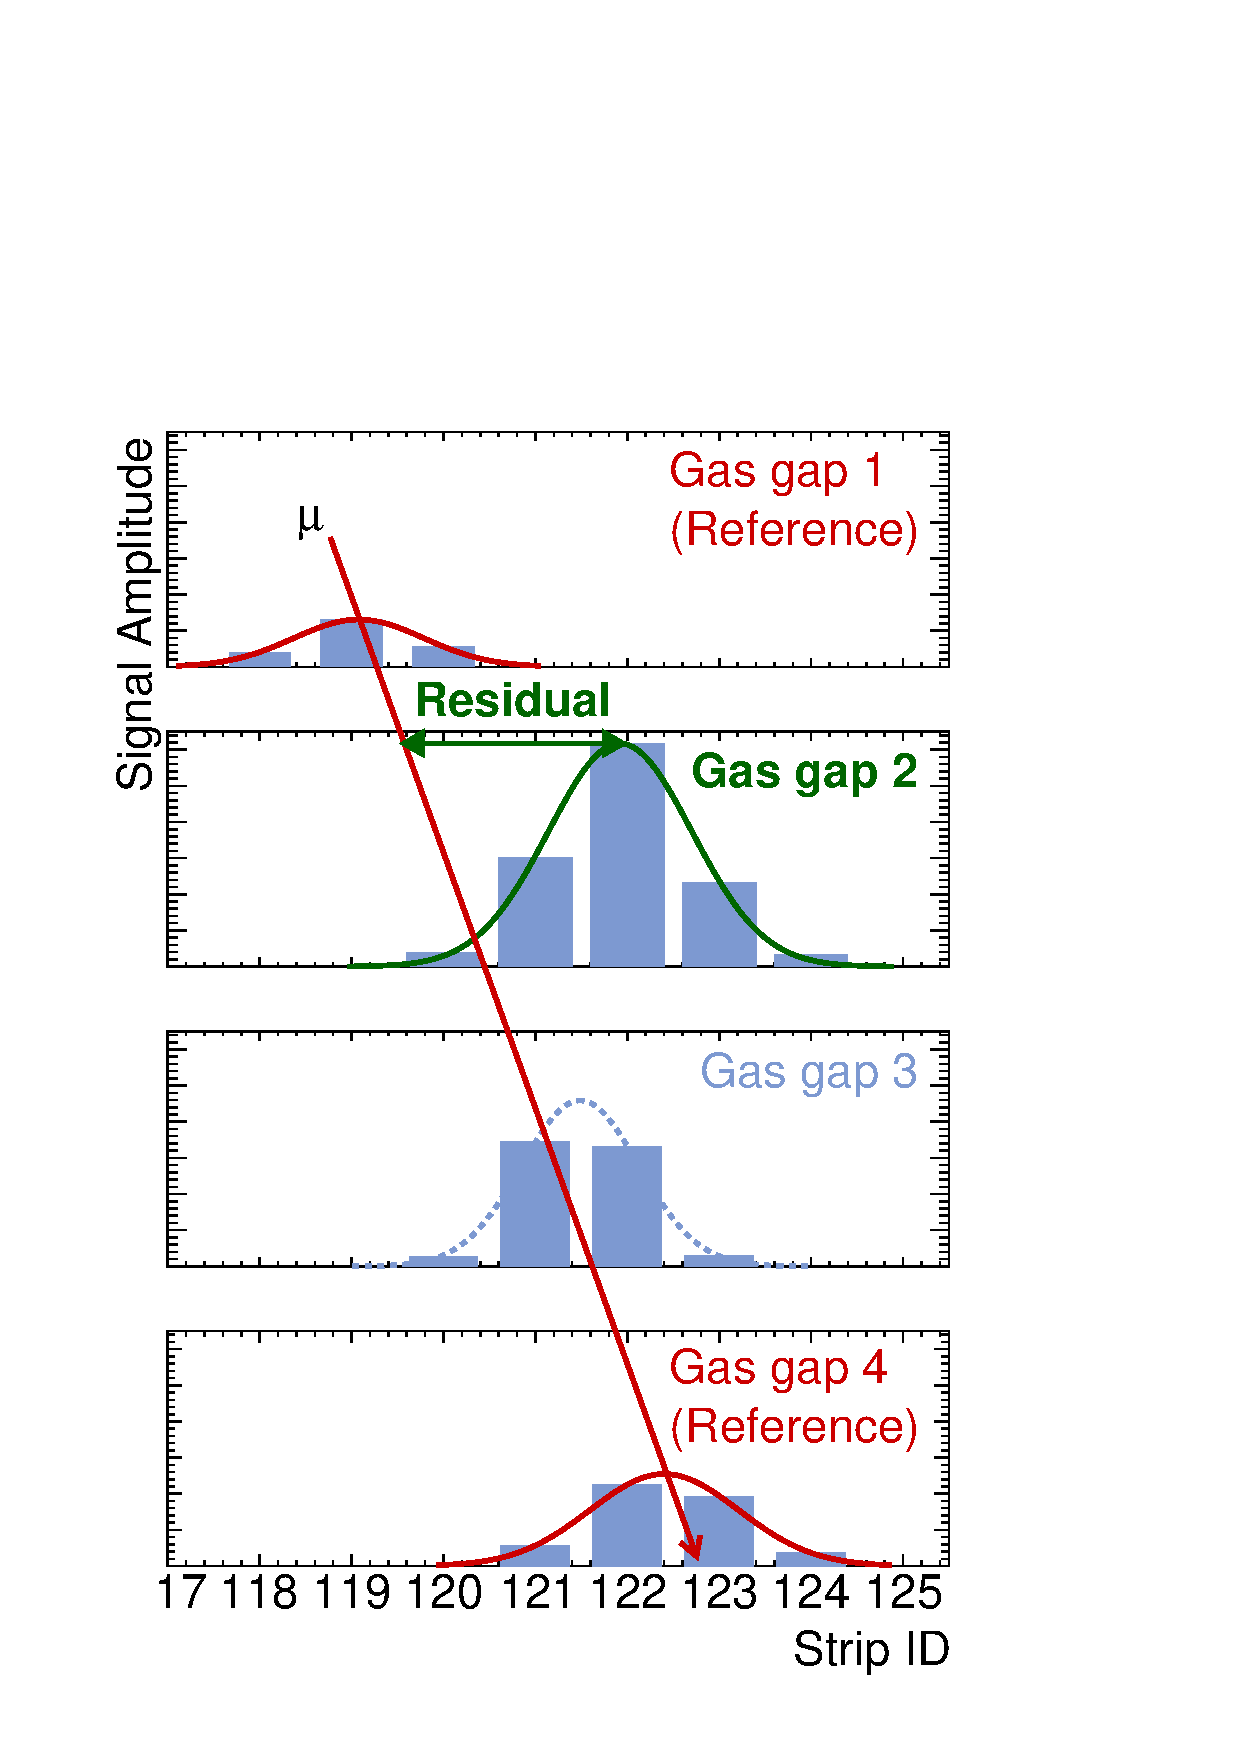
\includegraphics[width = 0.9\textwidth]{figures/figure_fake_event_display.pdf}
    \caption{Representation of a muon event recorded by an sTGC. The clusters are fit with a Gaussian and the mean is taken as the hit position. A track is built from the chosen reference layers, 1 and 4, and the residual calculated on layer 2. The clusters come from a real muon event, but their positions were modified to highlight the residual on layer 2.}
    \label{fig:fake_event_display}
\end{figure}

\begin{figure}
\centering
\begin{subfigure}{.5\textwidth}
  \centering
  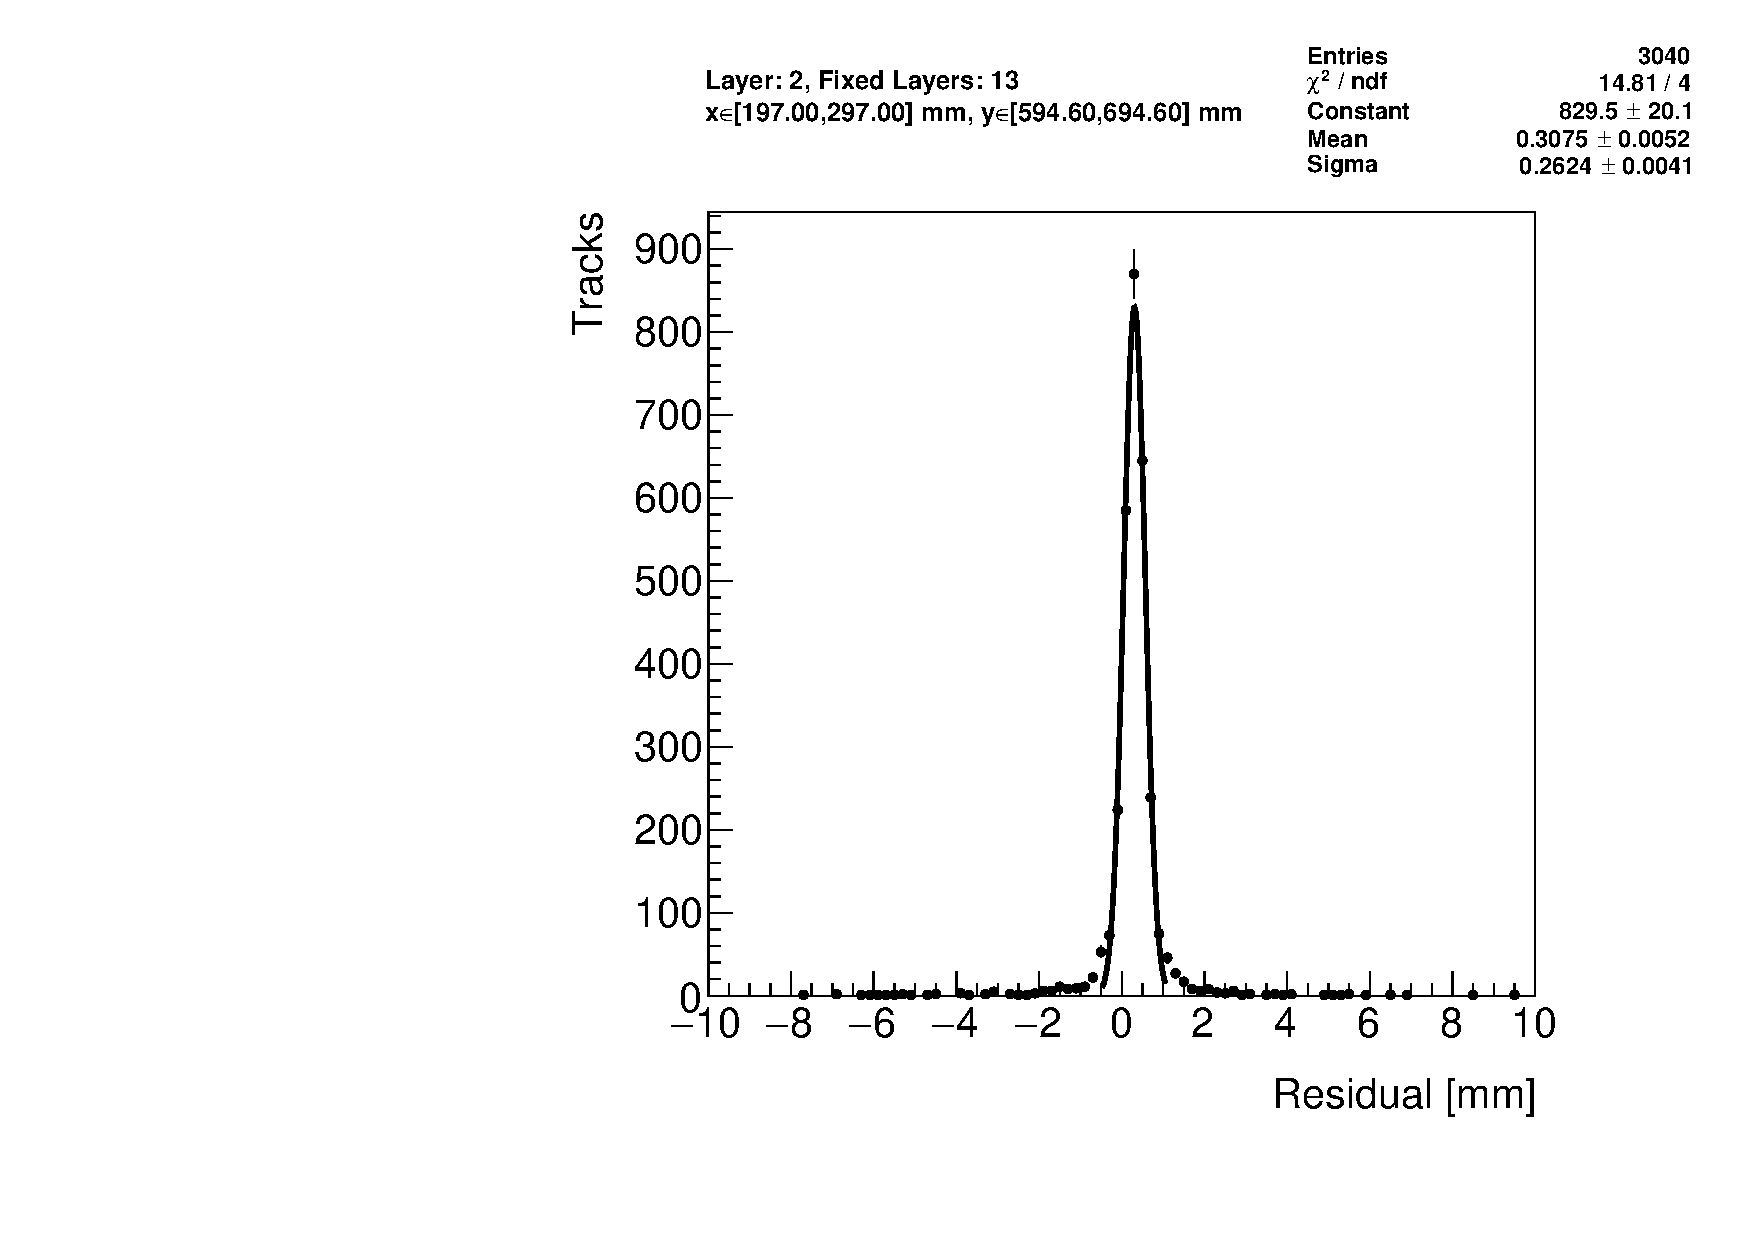
\includegraphics[width=\linewidth]{figures/figure_res_dist_QL2P11_3100V_2021-08-05_xbin_12_ybin_7_layer2_fixedlayers13.pdf}
  \caption{Tracks on layer 2, reference layers 1 and 3.}
  \label{fig:res_dist_L2_F13}
\end{subfigure}%
\begin{subfigure}{.5\textwidth}
  \centering
  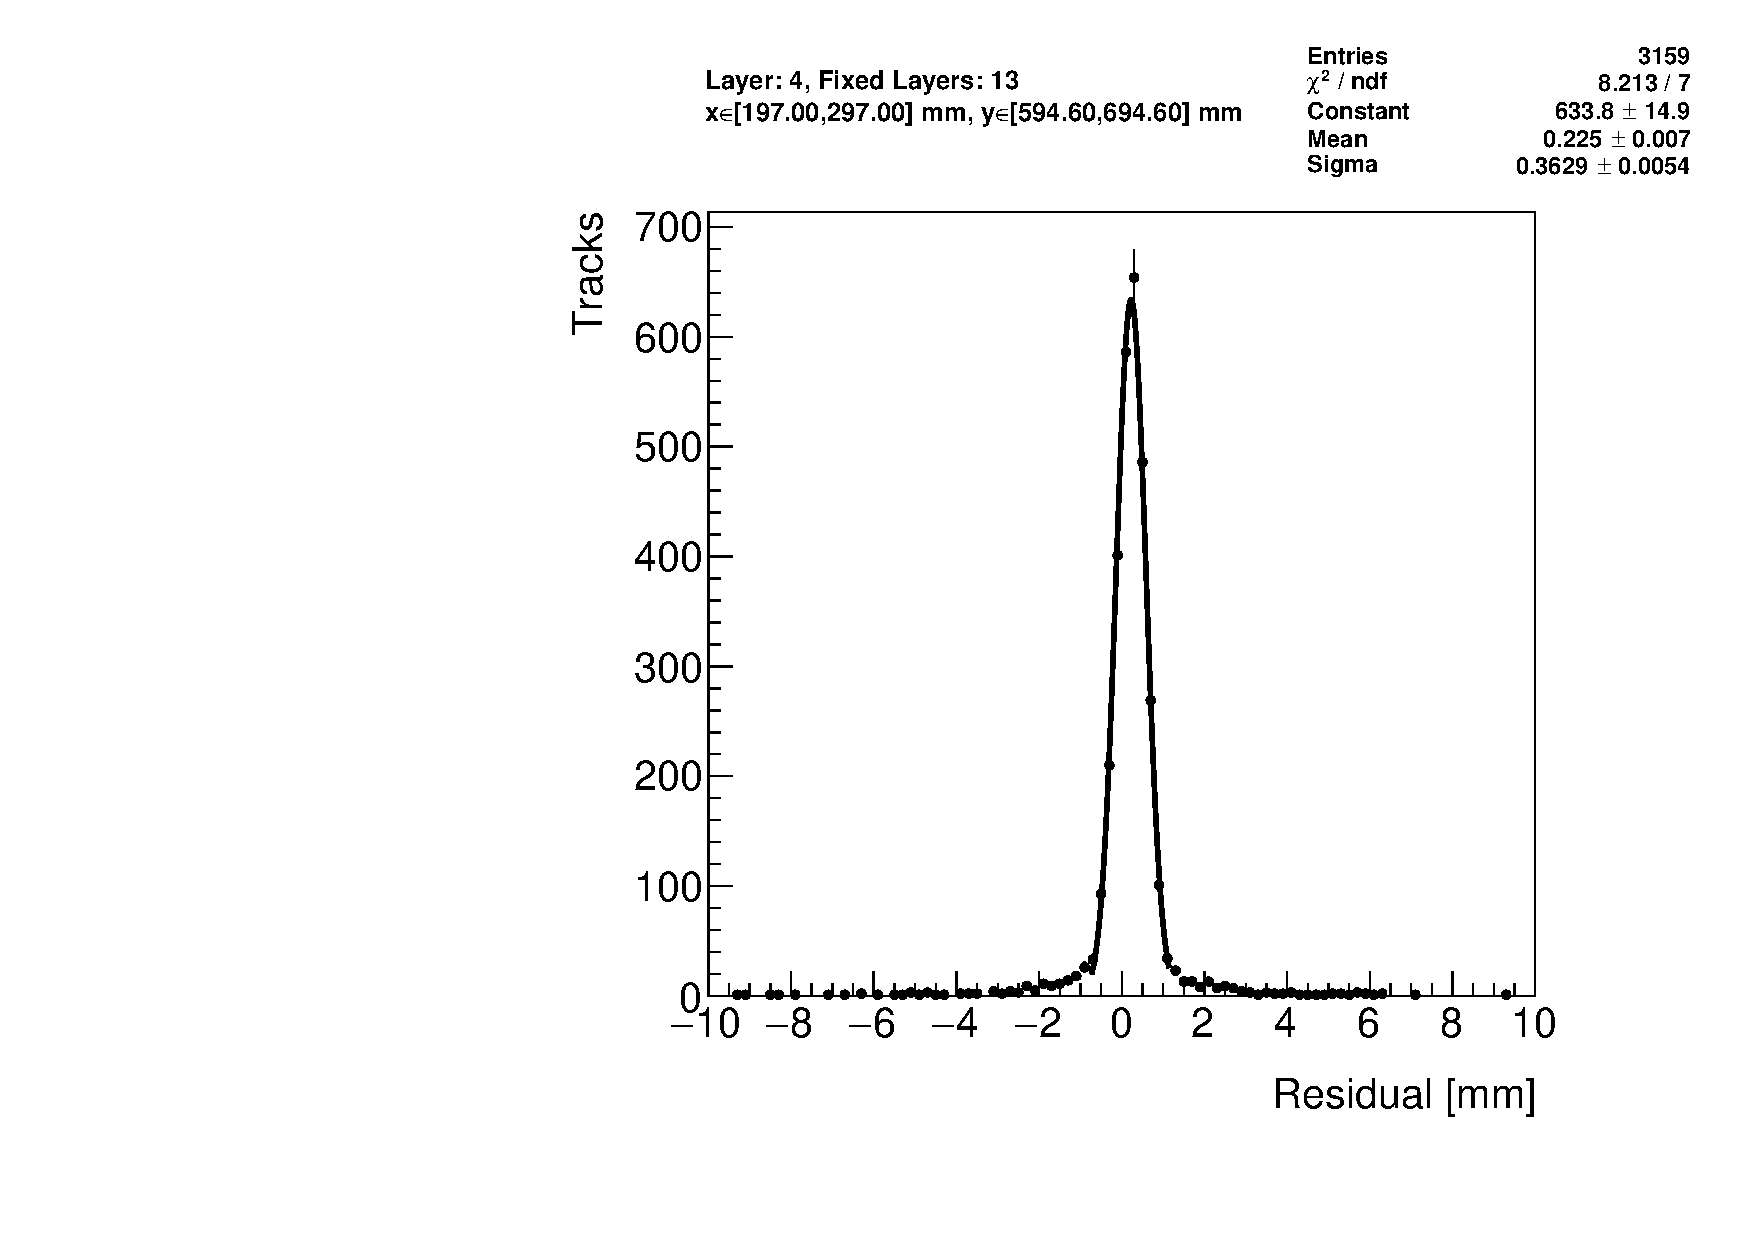
\includegraphics[width=\linewidth]{figures/figure_res_dist_QL2P11_3100V_2021-08-05_xbin_12_ybin_7_layer4_fixedlayers13.pdf}
  \caption{Tracks on layer 4, reference layers 1 and 2.}
  \label{fig:res_dist_L4_F12}
\end{subfigure}
\caption{Residual distribution in the region $x\in\left[197, 297\right],  y\in\left[594.6, 694.6\right] mm$ (100 mm by 100 mm area) for two different tracking combinations. }
\label{fig:res_dist}
\end{figure}

The residual distributions were wider for tracking combinations where the extrapolation lever arm was largest. In general, residual means calculated with geometrically less favourable tracking combinations have larger statistical and systematic uncertainties. The bin size of \SI{200}{\micro\meter} for the distributions shown in figure~\ref{fig:res_dist} was chosen based on the uncertainty on residuals calculated from tracks on layer 4 (1) built from hits on layers 1 and 2 (3 and 4) given a cluster y-position uncertainty of \SI{60}{\micro\meter} (appendix~\ref{appendix:clustering}), since these tracks yield residuals with the largest uncertainties.

A gaussian fit was used to extract the mean of the residual distributions. Theoretically, a double gaussian distribution is more apt, but for this analysis the gaussian fit was sufficient, as discussed in appendix~\ref{appendix:systematics_res_fit_fcn}.

The area of the region of interest was \SI{100}{\milli\meter} by \SI{100}{\milli\meter}. The size balanced the amount of tracks falling in the region of interest to give sufficient statistics to the local residual distributions, while being smaller than the order on which misalignments were expected to effect the local offsets significantly. "Significantly" in this context was defined based on the distance in $x$ that a large but possible rotation of \SI{1000}{\micro\radian} would change the local offset by more than \SI{50}{\micro\meter}, which is half the required position resolution of the sTGCs~\cite{nsw_tdr}.

It is only possible to calculate relative local offsets with cosmics data because there was no external reference to measure positions on all layers with respect to. As an example, assuming that the residual on layer 2 in figure~\ref{fig:fake_event_display} is representative of the relative local offset, the residual on layer 2 could be caused by layer 2 being misaligned from nominal, but it could also be caused by layers 1 and 4 being misaligned from nominal while layer 2 is in its expected position! Any number of combinations of local offsets on layers 1, 2 and 4 could produce the residual on layer 2. The value of relative local offset measurements will be shown and discussed throughout this work.

% --------------------------------------------------
\section{Visualizing relative misalignments between layers}
% --------------------------------------------------

The mean of residuals was extracted for regions across entire quadruplet layers for every tracking combination to get a picture of the relative misalignments between layers. 

\begin{figure}
\centering
\begin{subfigure}{0.85\textwidth}
  \centering
  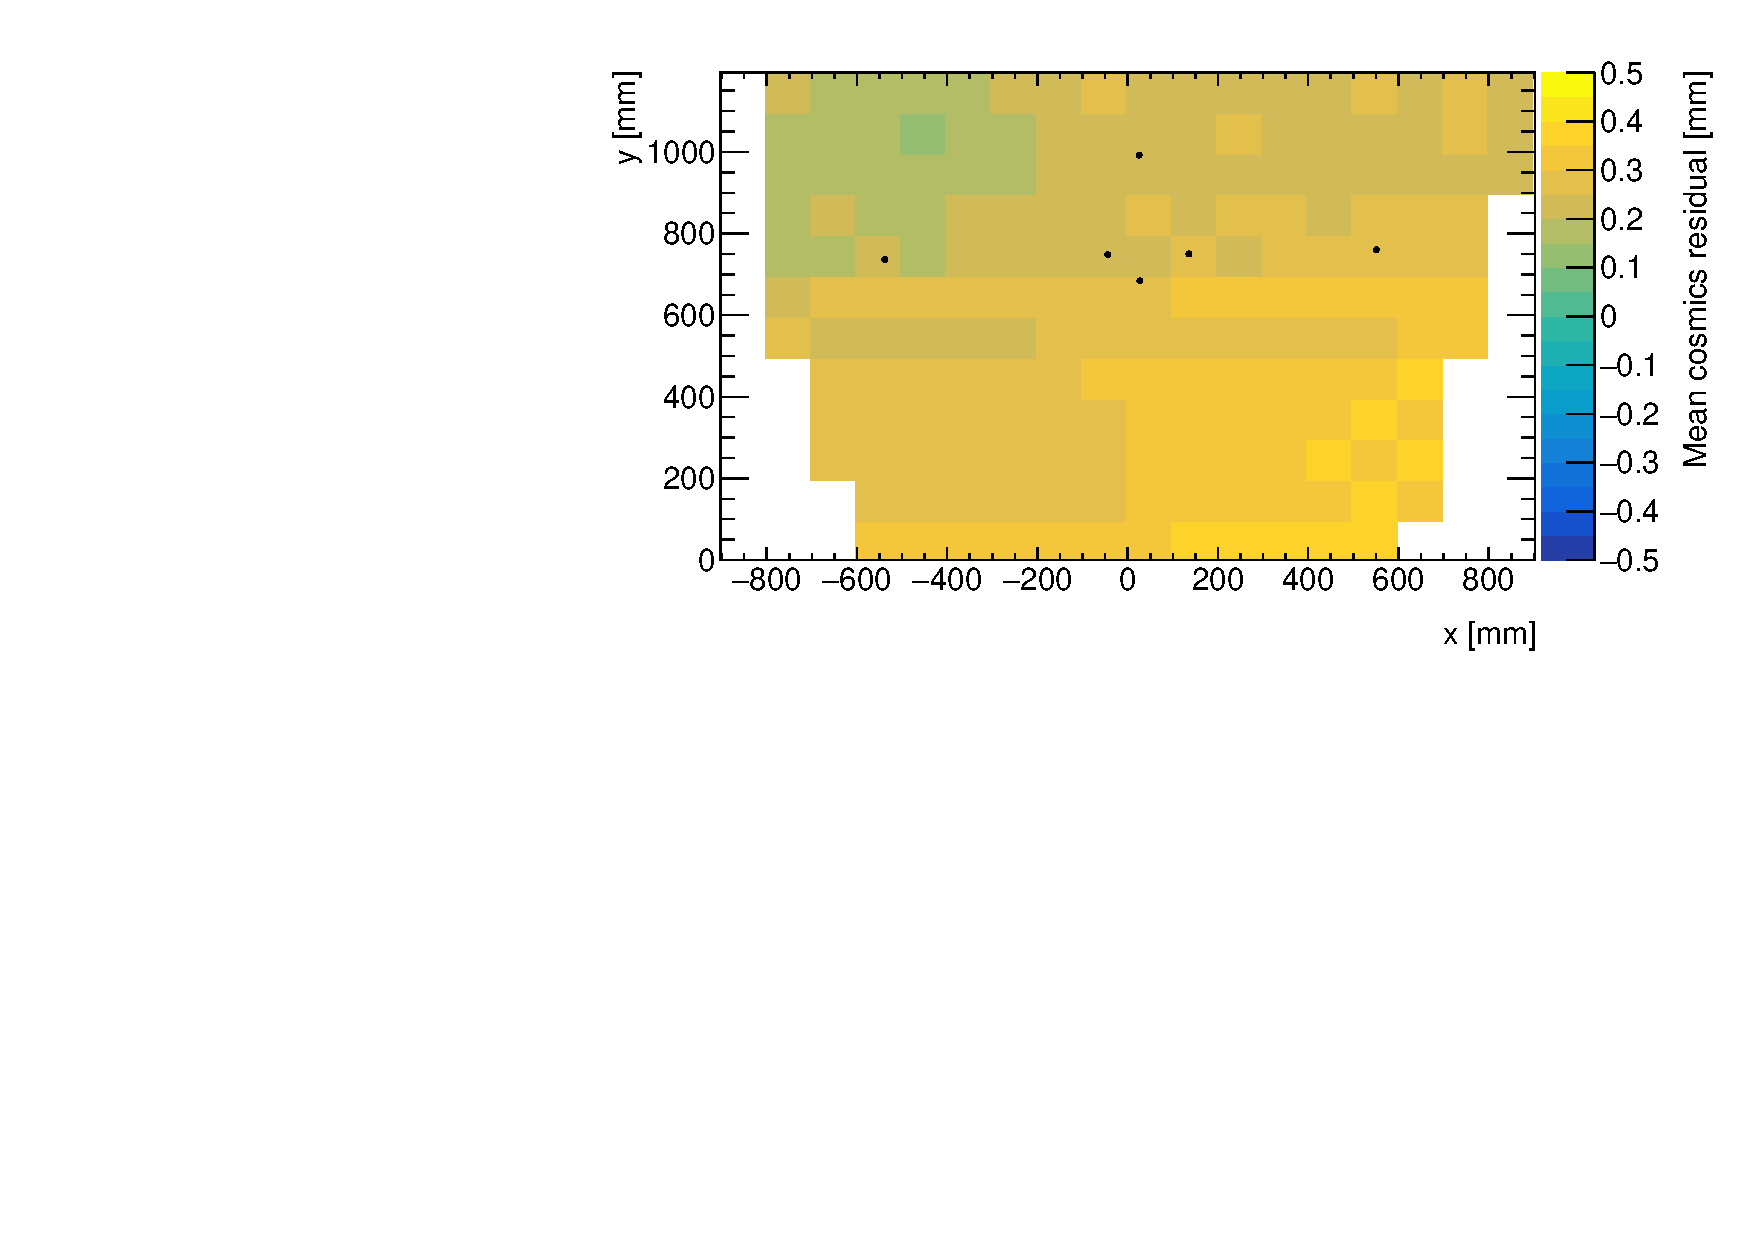
\includegraphics[width=\linewidth]{figures/figure_QL2P11_3100V_2021-08-05_fit_means_xray_overlay_layer2_fixedlayers13.pdf}
  \caption{Mean of residuals for tracks on layer 2, reference layers 1 and 3.}
  \label{fig:res_mean_th2_L2_F13}
\end{subfigure}%
\vspace*{\floatsep}
\begin{subfigure}{0.85\textwidth}
  \centering
  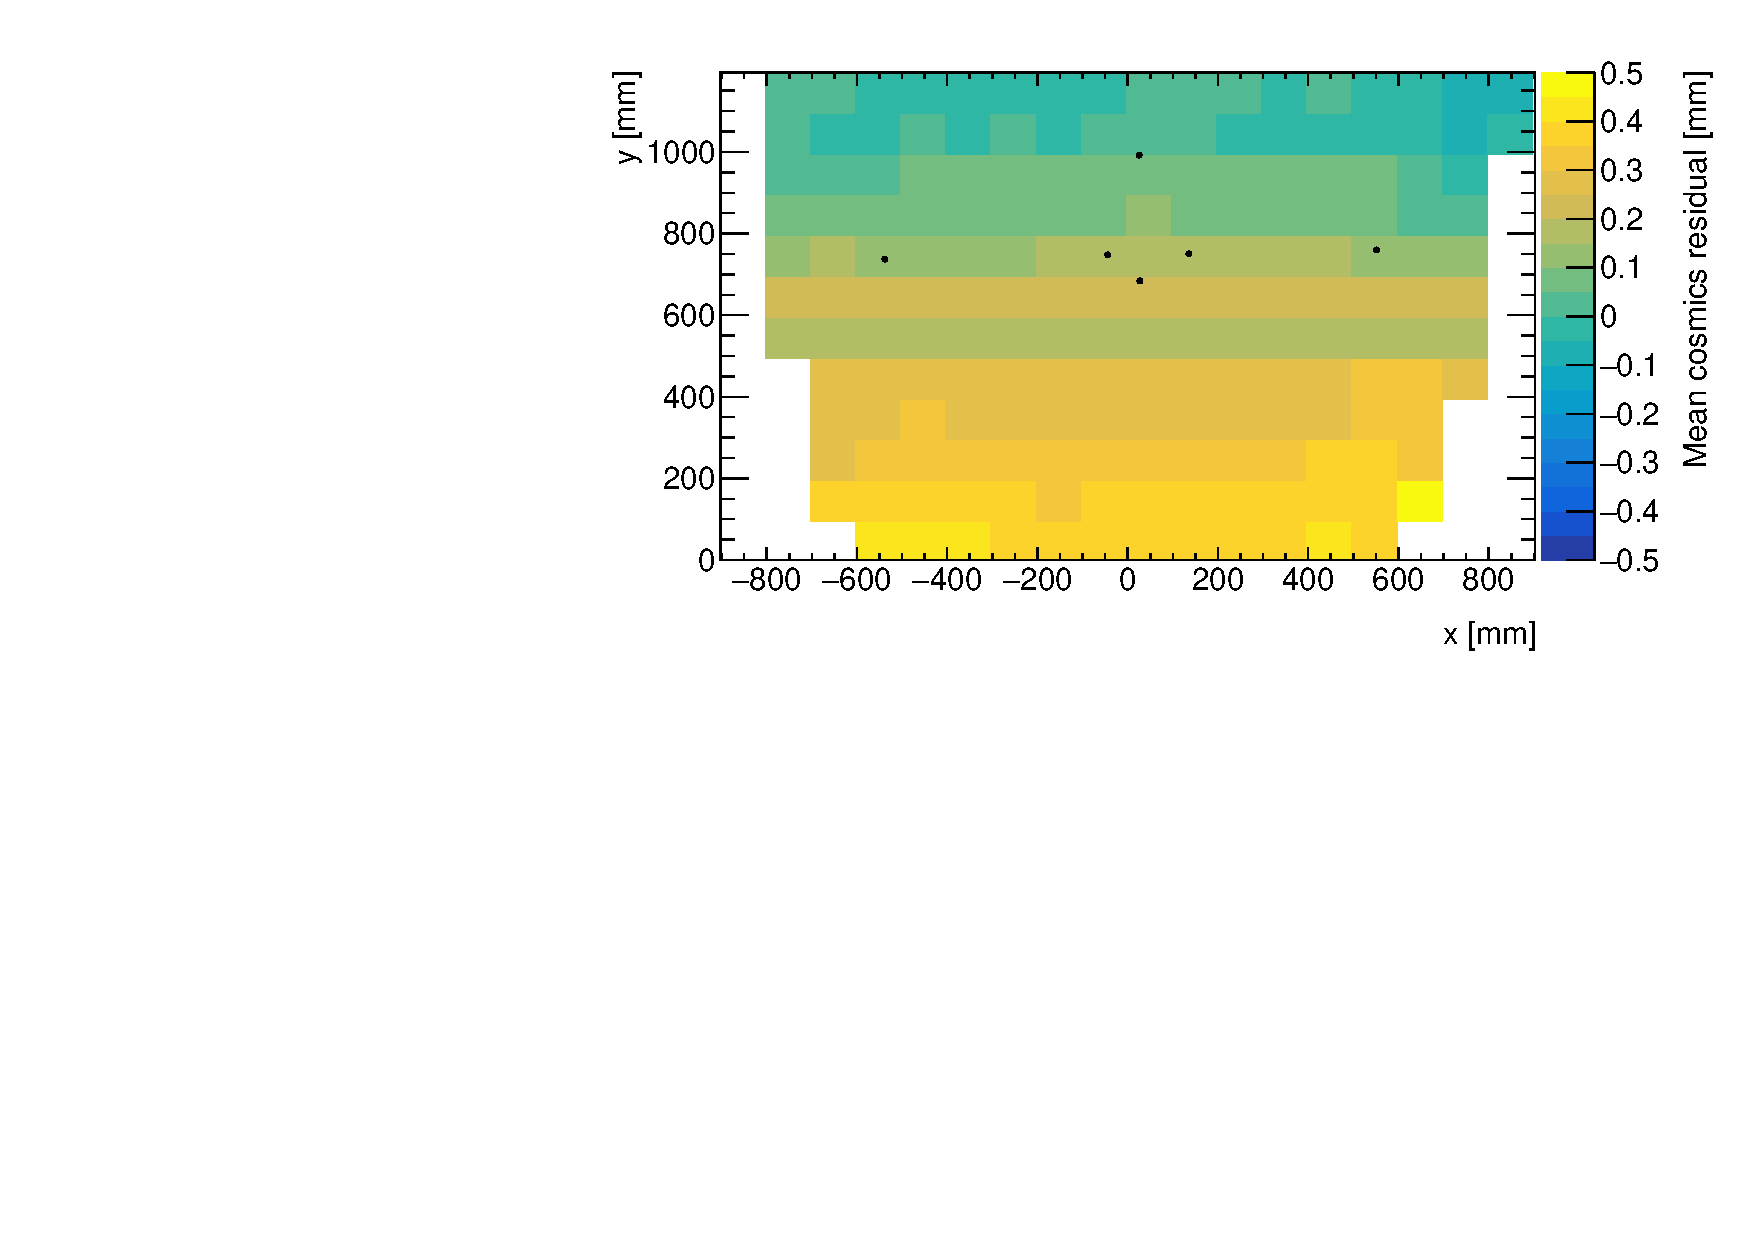
\includegraphics[width=\linewidth]{figures/figure_QL2P11_3100V_2021-08-05_fit_means_xray_overlay_layer4_fixedlayers13.pdf}
  \caption{Mean of residuals for tracks on layer 4, reference layers 1 and 3.}
  \label{fig:res_mean_th2_L4_F13}
\end{subfigure}
\caption{Mean of residuals in each \SI{100}{\milli\meter} by \SI{100}{\milli\meter} bin over the area of the quad layer for QL2.P.11. The black points represent x-ray survey positions, discussed in chapter~\ref{chap:comparison}.}
\label{fig:res_mean_th2}
\end{figure}

Figure~\ref{fig:res_mean_th2} contains the mean of residuals on layers 2 and 4 with tracking reference layers 1 and 3. Many of the residual means are non-zero, and change smoothly over the layer, indicating that there are relative misalignments. Given that the residual mean changes with $x$ in figure~\ref{fig:res_mean_th2_L2_F13}, there is likely a rotation of layer 2 with respect to layers 1 and 3, combined with an offset of the entire layer. For layer 4 in figure~\ref{fig:res_mean_th2_L4_F13}, perhaps there is a scaling~\cite{carlson_results_2019} of the strip pattern with respect to layers 1 and 3. The interpretation of the patterns in the residual means depends on the choice of misalignment model.

% --------------------------------------------------
\section{Systematic uncertainty in cosmic residual means}
% --------------------------------------------------

The statistical uncertainty on the local residual means was typically around \SI{10}{} - \SI{20}{\micro\meter}, and appendix~\ref{appendix:statistics} shows that the analysis was not statistically limited by the number of triggers collected for each quadruplet. The systematic uncertainties were more significant. 

Systematic uncertainties were assigned per tracking combination as the RMS of the distribution of the difference in local residual means each calculated with a different analysis choice. For example, the RMS associated with fitting the local residual distributions with a Gaussian or double Gaussian is \SI{25}{\micro\meter} for the geometrically least favourable tracking combinations and the distribution is shown in appendix~\ref{appendix:systematics_res_fit_fcn}. For geometrically similar tracking combinations (like: tracks on layer 1 built from hits on layers 3 and 4, and tracks on layer 4 built from hits on layers 1 and 2), the systematic uncertainty was assigned as the average RMS for both.

Other choices were whether to use data collected at 2.9~kV or 3.1~kV; what cluster fitting algorithm to use; and whether or not to apply a differential non-linearity (DNL) correction to the cluster y-positions. A systematic uncertainty was assigned using the method above to account for the effect of each choice. The reasons for each choice are listed below.

Data taken at 3.1~kV was used over 2.9~kV because the strip and wire tracking efficiency increases with higher voltage~\cite{lefebvre_thesis} (appendix~\ref{appendix:systematics_2900V_vs_3100V}).

The \package{Minuit2} package~\cite{hatlo_developments_2005} was used to fit clusters over Guo's method~\cite{guo_simple_2011} because it provided automatic statistical uncertainty estimates and is the standard choice (appendix~\ref{appendix:systematics_cluster_fit_fcn}).

The DNL correction was not applied because its effect on the residual means was negligible (appendix~\ref{appendix:systematics_dnl}).

A summary of the systematic uncertainties assigned for each tracking combination is given in table~\ref{tab:sys_uncerts}.

%TODO : Maybe just make the table have the total sys uncertainty, and put the breakdown at the end of appendix:systematics
%\begin{center}
\begin{table}

\begin{tabularx}{\textwidth} {
 | >{\raggedright\arraybackslash}X 
 | >{\raggedright\arraybackslash}X 
 | >{\raggedright\arraybackslash}X
 | >{\raggedright\arraybackslash}X 
 | >{\raggedright\arraybackslash}X 
 | >{\raggedright\arraybackslash}X 
 | >{\raggedright\arraybackslash}X 
 | >{\raggedright\arraybackslash}X 
 | >{\raggedright\arraybackslash}X | }
 
 \hline
 \textbf{Layer} & \textbf{Fixed layer 1} & \textbf{Fixed layer 2} & \textbf{\ref{appendix:systematics_res_fit_fcn}} & \textbf{\ref{appendix:systematics_2900V_vs_3100V}} & \textbf{\ref{appendix:systematics_cluster_fit_fcn}} & \textbf{\ref{appendix:systematics_dnl}} & \textbf{Total} \\ 
 \hline
 \hline 
 3 & 1 & 2 & 0.010 & 0.041 & 0.018 & 0.008 & \textbf{0.047} \\
 \hline
    4 & 1 & 2 & 0.025 & 0.091 & 0.027 & 0.012 & \textbf{0.098} \\
 \hline
    2 & 1 & 3 & 0.008 & 0.020 & 0.012 & 0.003 & \textbf{0.025} \\
 \hline
    4 & 1 & 3 & 0.007 & 0.042 & 0.013 & 0.005 & \textbf{0.044} \\
 \hline
    2 & 1 & 4 & 0.006 & 0.035 & 0.012 & 0.005 & \textbf{0.038} \\
 \hline
    3 & 1 & 4 & 0.006 & 0.035 & 0.012 & 0.005 & \textbf{0.038} \\
 \hline
    1 & 2 & 3 & 0.010 & 0.041 & 0.018 & 0.008 & \textbf{0.047} \\
 \hline
    4 & 2 & 3 & 0.010 & 0.041 & 0.018 & 0.008 & \textbf{0.047} \\
 \hline
    1 & 2 & 4 & 0.007 & 0.042 & 0.013 & 0.005 & \textbf{0.044} \\
 \hline
    3 & 2 & 4 & 0.008 & 0.020 & 0.012 & 0.003 & \textbf{0.025} \\
 \hline
    1 & 3 & 4 & 0.025 & 0.091 & 0.027 & 0.012 & \textbf{0.098} \\
 \hline
    2 & 3 & 4 & 0.010 & 0.041 & 0.018 & 0.008 & \textbf{0.047} \\
 \hline
 
\end{tabularx}
\caption{Systematic uncertainty assigned for each analysis option, detailed in appendix~\ref{appendix:systematics}.}
\label{tab:sys_uncerts}
\end{table}

The uncertainty in each mean cosmics residual was assigned as the sum in quadrature of the statistical uncertainty in the mean and the appropriate systematic uncertainty for the tracking combination. Given that the uncertainty in the mean cosmics residuals is lesser than or near to the order of the required position resolution of the sTGCs (\SI{100}{\micro\meter}~\cite{nsw_tdr}) the cosmic residual means are relevant input for alignment studies.

% --------------------------------------------------
\section{The x-ray method}
% --------------------------------------------------
\label{x_ray}

%TODO : consistently call the x-ray centroids the "x-ray beam profile centers"

Work on characterizing relative misalignments between quadruplet layers is ongoing~\cite{zhao_cosmic_2019}, \textcolor{red}{(Can I cite John's thesis-in-progress?)} but what is required are the absolute strip positions with respect to their nominal position in the ATLAS analysis coordinate system \textcolor{red}{to be input into Athena(?)}. Somehow, absolute misalignment parameters must be derived to create a model of absolute strip positions - which is not possible with the cosmics dataset. Absolute local offset measurements were done by the so-called x-ray method~\cite{lefebvre_precision_2020}. The x-ray tests were performed after the quadruplets arrived at CERN and were assembled into wedges. Essentially, an x-ray gun was attached to one of the source plates glued to the surface of the wedge (figure~\ref{fig:xray_setup}), and the beam profile recorded by the strips.

\begin{figure}
    \centering
    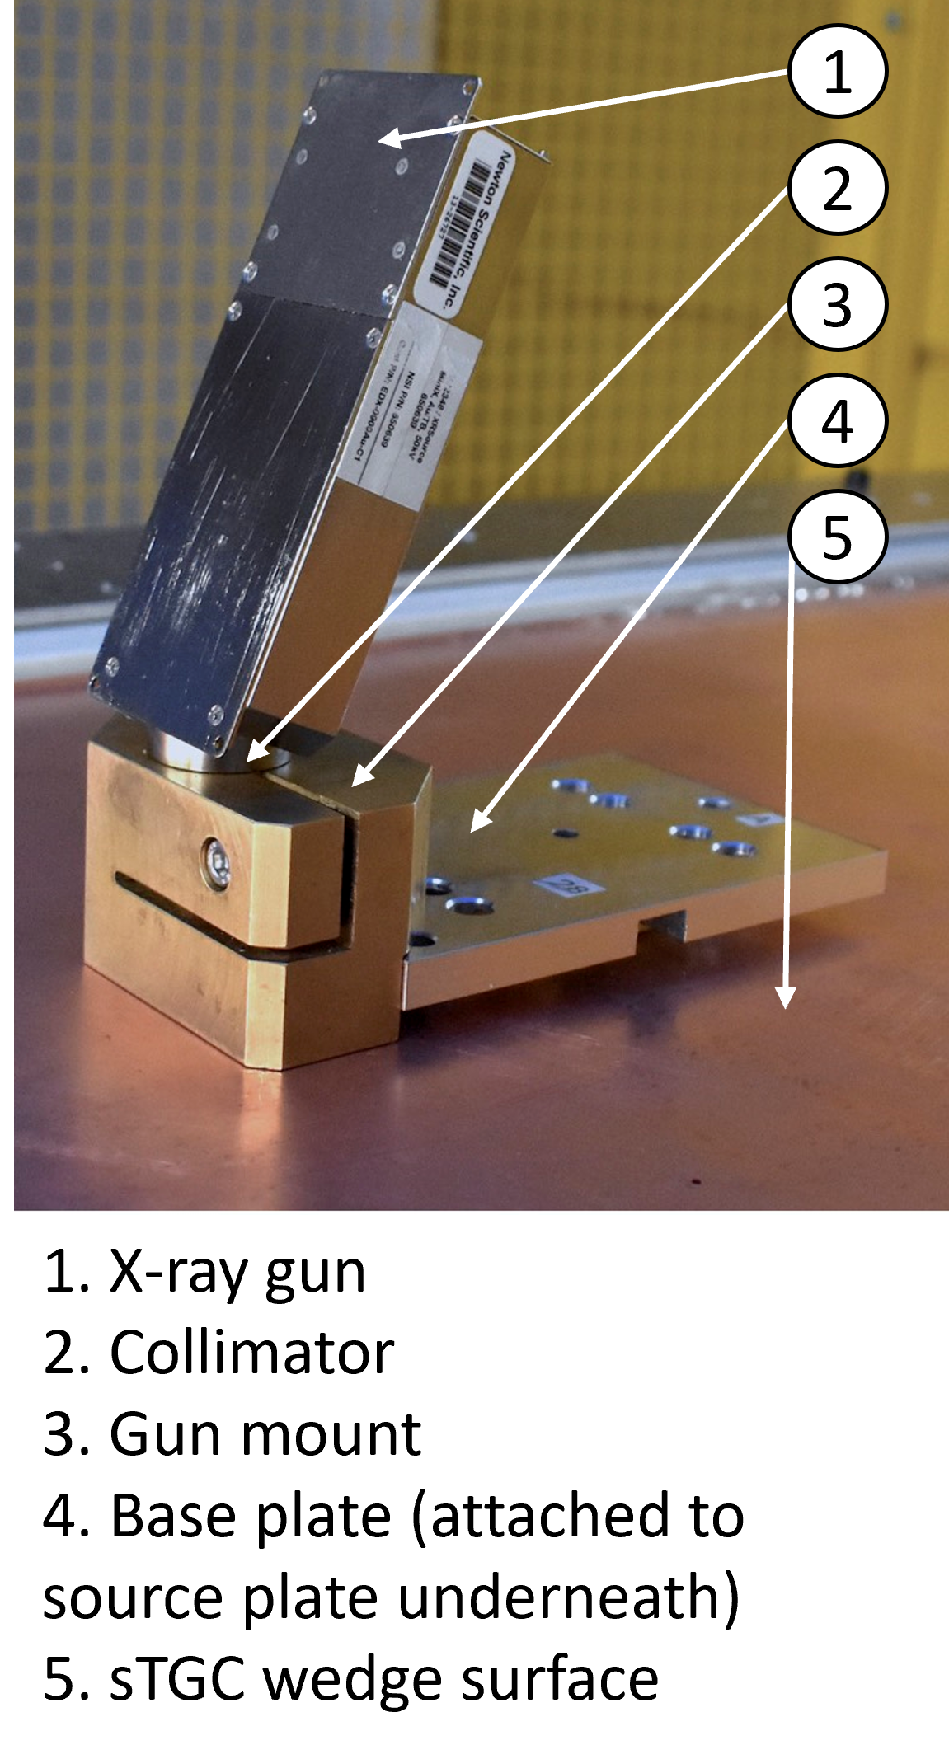
\includegraphics[width = 0.5\textwidth]{figures/figure_xray_setup.pdf}
    \caption{The x-ray gun mounted to the alignment platform on the surface of the wedge. Adapted from \copyright  CERN for the benefit of the ATLAS collaboration. CC-BY-4.0 license.}
    \label{fig:xray_setup}
\end{figure}

% During ATLAS operation, the position of the source plates will be monitored using the new alignment system~\cite{nsw_tdr}. Therefore, their position will be known in the absolute ATLAS coordinate system. 

The gun produced x-rays of 7 - \SI{15}{\kilo\electronvolt} that were collimated before reaching the surface of the wedge. The x-rays mostly interacted with the wedge's copper electrodes and gold-plated tungsten wires via the photo effect. \textcolor{red}{The resulting photoelectrons ionized the CO$_2$ in the gap, which resulted in detectable Townsend avalanches -- \textit{is it really avalanches or just electrons drifting back?}}. The beam profile was captured by the distribution of cluster positions. A typical beam profile is shown in figure~\ref{fig:xray_beam_profile}.

%TODO : What separates a delta ray and a photoelectron?

\begin{figure}
    \centering
    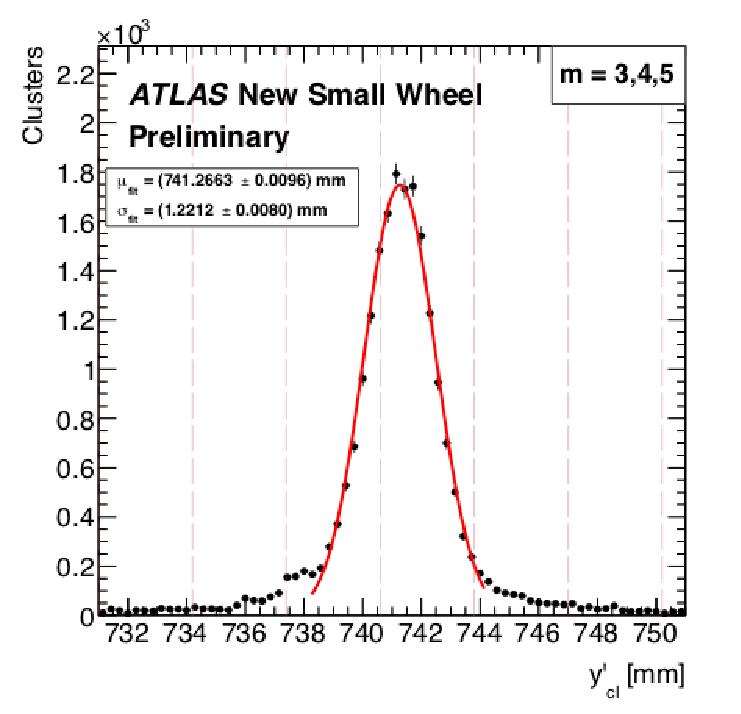
\includegraphics[width = 0.5\textwidth]{figures/figure_xray_beam_profile.pdf}
    \caption{Distribution of x-ray cluster mean positions after the analysis cuts and corrections. The strip cluster multiplicity, $m$, was limited to 3, 4 and 5. The red line is a Gaussian fit of the distribution and the pink lines denote the edges of the strips. Adapted from \copyright CERN for the benefit of the ATLAS collaboration. CC-BY-4.0 license.}
    \label{fig:xray_beam_profile}
\end{figure}

The mean of the cluster position distribution was taken as the x-ray beam profile center. The expected center was calculated assuming a wedge with nominal geometry given the gun position. The difference between the expected and reconstructed beam profile center is a measure of the local offset. Applying the logic of equation~\ref{eqn:local_translation} to the beam profile, the fitted mean acts as $y$, the expected center is $y_{nom}$ and the local offset is $d_{local}$ as before. The x-ray local offsets  give the absolute local position of the strip pattern with respect to the source plates. Since the position of the source plates will be monitored by the alignment system in ATLAS~\cite{nsw_tdr}, the local position of the strip pattern can be known in the ATLAS coordinate system for every position where x-ray data was taken.

The main advantage of the x-ray dataset over the cosmics dataset is that absolute local offsets are measurable thanks to the reference frame provided by the source plates. However, the systematic uncertainty on the x-ray offsets is large: \SI{120}{\micro\meter} was accepted by the collaboration. The cuts and corrections applied to the x-ray data that motivate the uncertainty are detailed in Lefebvre, 2020~\cite{lefebvre_precision_2020}. In addition, local offset measurements were limited to the positions of the alignment platforms; only 10 - 20 positions were surveyed for each wedge. Therefore, validating the x-ray measurements and seeing how they can be improved is important because of the uncertainty in and incompleteness of the dataset. How the cosmics dataset was used for this purpose is discussed in chapter~\ref{chap:comparison}. 
\input{chapters/4_the_xray_method}
% ==================================================
% CHAPTER 4: Validating x-ray alignment parameters with cosmic muon data %
% ==================================================

\chapter{Validating x-ray alignment parameters with cosmic muon data}

% --------------------------------------------------
\section{Presentation of theoretical method for comparison}
% --------------------------------------------------

The goal of this work is to validate the alignment parameters extracted from the x-ray data with cosmics data. 
% maybe delete this entire section if it is already elsewhere.

The x-ray parameters are in a useful coordinate system but the nature of x-ray events lead to large clusters and delta rays \cite{lefebvre_precision_2020}, and far less clusters are collected than in cosmics. Cosmic muon data is cleaner by the nature of the interaction of muons and less statistically limited, but the relative coordinate system cannot be used to calculate misalignment parameters. Therefore, it is desirable to validate the alignment parameters extracted from the x-ray dataset with cosmics data.

There is no reason the method of two-layer tracking cannot be applied to the x-ray data as well. The x-ray beam centroid on each layer can be taken as a track position, the track evaluated on another layer, then the residual calculated. As with cosmic muon clusters, the cluster position mean should be systematically offset by the local misalignment of the strip pattern, so when tracked the x-ray track residual should match the mean of cosmic track residuals. 



%----------------------------------------------------------------------
% END MATERIAL
% Bibliography, Appendices, Index, etc.
%----------------------------------------------------------------------

% Bibliography

% The following statement selects the style to use for references.  
% It controls the sort order of the entries in the bibliography and also the formatting for the in-text labels.
% Tony used unsrt in his PhD thesis
\bibliographystyle{unsrt}
% This specifies the location of the file containing the bibliographic information.  
% It assumes you're using BibTeX to manage your references (if not, why not?).
% \cleardoublepage % This is needed if the "book" document class is used, to place the anchor in the correct page, because the bibliography will start on its own page.
% Use \clearpage instead if the document class uss the "oneside" argument
\phantomsection  % With hyperref package, enables hyperlinking from the table of contents to bibliography             
% The following statement causes the title "References" to be used for the bibliography section:
\renewcommand*{\bibname}{References}

% Add the References to the Table of Contents
\addcontentsline{toc}{chapter}{\textbf{References}}

\bibliography{thesis}
% Tip: You can create multiple .bib files to organize your references. 
% Just list them all in the \bibliogaphy command, separated by commas (no spaces).

% The following statement causes the specified references to be added to the bibliography even if they were not cited in the text. 
% The asterisk is a wildcard that causes all entries in the bibliographic database to be included (optional).
\nocite{*}
%----------------------------------------------------------------------

% Appendices

% The \appendix statement indicates the beginning of the appendices.
\appendix
% Add an un-numbered title page before the appendices and a line in the Table of Contents
\chapter*{APPENDICES}
\addcontentsline{toc}{chapter}{APPENDICES}
% Appendices are just more chapters, with different labeling (letters instead of numbers).
% ==================================================
% Appendix: Uncertainty in cluster positions %
% ==================================================

%TODO : Organize figure positioning once you're done writing. 

\chapter[Cluster position uncertainty]{Uncertainty in cluster positions}
\label{appendix:clustering}

% Cluster def
% Cluster x from wires, cluster y from strips
% Cluster x uncertainty
% Cluster y statistical uncertainty
% Cluster y systematic uncertainty depending on choice of fitting algorithm

%TODO : What causes variation in cluster size? Why do we see changes in relative cluster size populations between 2900 V and 3100 V data? Benoit's thesis, page 36, references. Need this to correct red sentence.
A cluster is a series of contiguous strip channels on a layer with non-zero amplitude, all part of the same trigger and having the same event number~\cite{lefebvre_thesis}. \textcolor{red}{Clusters result from a muon ionizing gas in the gap, and the number of strips in the corresponding cluster depends on the angle of the track and the gain (operating voltage)}. The peak-detector-output (PDO) of the signal on each strip of a cluster is fit with a Gaussian. The y-position of a particle as it passed through the layer is mean of the cluster, referred to here as the hit position.

The uncertainty assigned to the hit position affects the uncertainty in the calculated residuals, and so informs the appropriate bin width for the residual distributions. There is a statistical uncertainty in the hit position from the estimation of the Gaussian mean, but also a systematic uncertainty that depends on the fit algorithm used. 

The clusters were fit with Guo's method~\cite{guo_simple_2011} and Minuit2 for ROOT~\cite{hatlo_developments_2005}. The difference in cluster means between the two algorithms is shown in figure~\ref{fig:mu_reclustering_minus_mu_cosmics}.

%TODO : Make this figure pretty with a nicer text box?
\begin{figure}
    \centering
    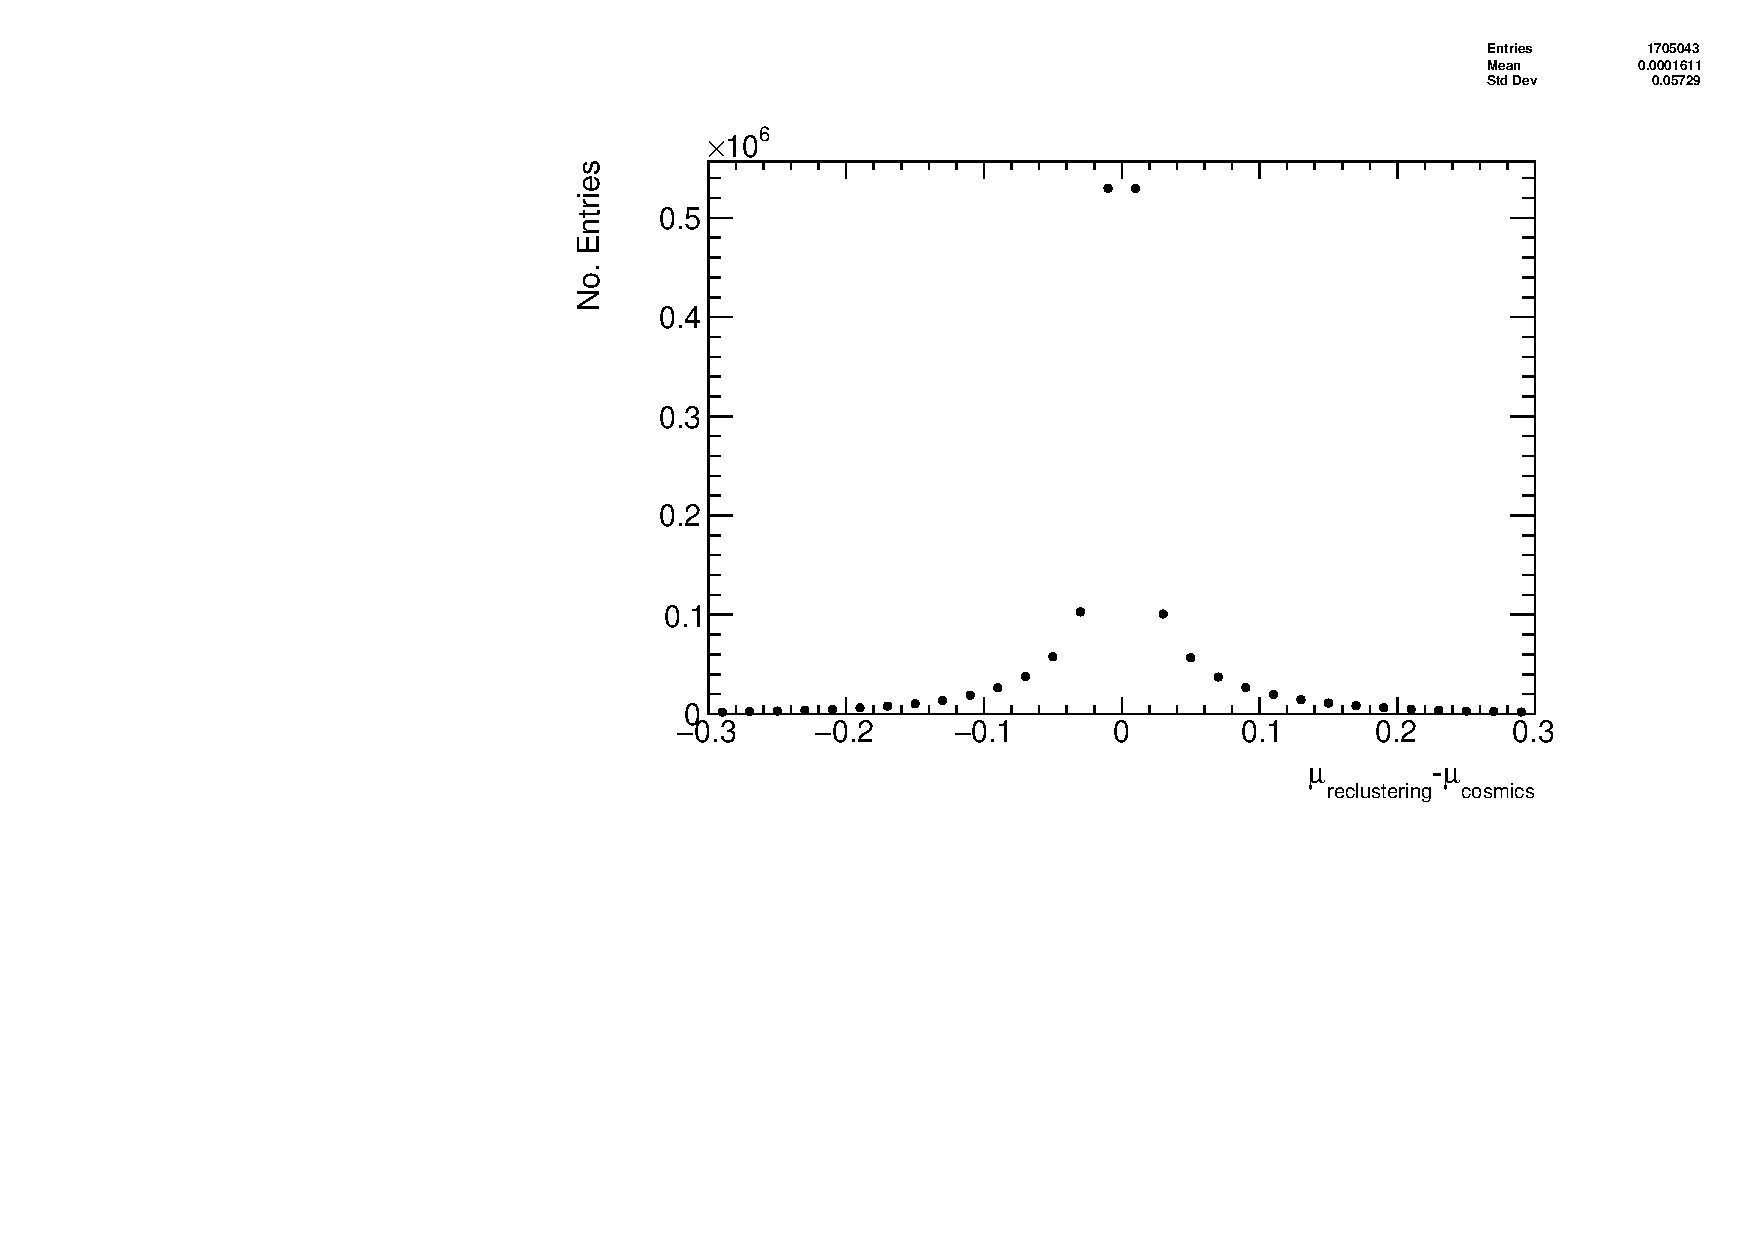
\includegraphics[width = 0.7\textwidth]{figures/figure_QL2P08_3100V_2021-05-21_reclustering_plots_mu_reclustering_minus_mu_cosmics.pdf}
    \caption{The difference between cluster means calculated with Guo's method~\cite{guo_simple_2011} in \package{tgc\_analysis/CosmicsAnalysis} and Minuit2 for ROOT~\cite{hatlo_developments_2005} in \package{strip\_position\_analysis/ReClustering} for data collected with QL2.P.8 at 3.1~kV.}
    \label{fig:mu_reclustering_minus_mu_cosmics}
\end{figure}

The RMS of the distribution in figure~\ref{fig:mu_reclustering_minus_mu_cosmics} is \SI{57}{\micro\meter}, which is much larger than the statistical uncertainty in the mean for the Minuit2 algorithm, which peaks around \SI{7}{\micro\meter}. An RMS of \SI{57}{\micro\meter} is common for data taken with most quadruplets at 3.1~kV. Therefore, the uncertainty in the y-hit positions is assigned \SI{57}{\micro\meter}.

%TODO : How does this inform the residual distribution bin size?

The x position of the cluster is taken to be the center of the wire group with the maximum detected signal, since wire groups are wide enough that usually only one wire picks up the ionization avalanche. 

%TODO : How does this inform the area of the bins we take residual means in?

%TODO : How does reclustering affect residual means?

% ==================================================
% Appendix: Analysis Statistics %
% ==================================================

\chapter[Analysis statistics]{Study of cosmics for alignment analysis statistical uncertainty}
\label{appendix:statistics}
% Edit count: 0

% Plan:
% Quantity of interest is the Gaussian mean of the residual distribution in a region of interest.
% Typically, have 1 million triggers; for QS3.P.18 got 3.5 million triggers.
% See the drop off in peak residual mean error with more triggers (FIGURE).
% We are not statistically limited. Compare residual fits for L1 F34 between 1 million triggers and 3.5 million triggers: means don't change significantly.

Typically, one million triggers (cosmic muon events, noise, photons and $\delta$-rays) were collected for each Canadian quadruplet at McGill University, resulting in roughly half the number of viable tracks after cuts. For QS3.P.18, 3.5 million triggers were collected. To gauge the sensitivity of the analysis to the available statistics, partitions of this data with each with a different number of triggers were analyzed separately. Ultimately, the quantity of interest was the Gaussian mean of the residual distribution in regions of interest, so the peak in the distribution of the statistical uncertainty in the residual means for each area of interest for a specific tracking combination was used to gauge the quality of the analysis. How the peak in the residual mean uncertainty distribution changes with the number of triggers is shown in figure for tracks on layer 1 built from layers 3 and 4 \ref{fig:res_mean_uncert_vs_triggers}. 

\begin{figure}
    \centering
    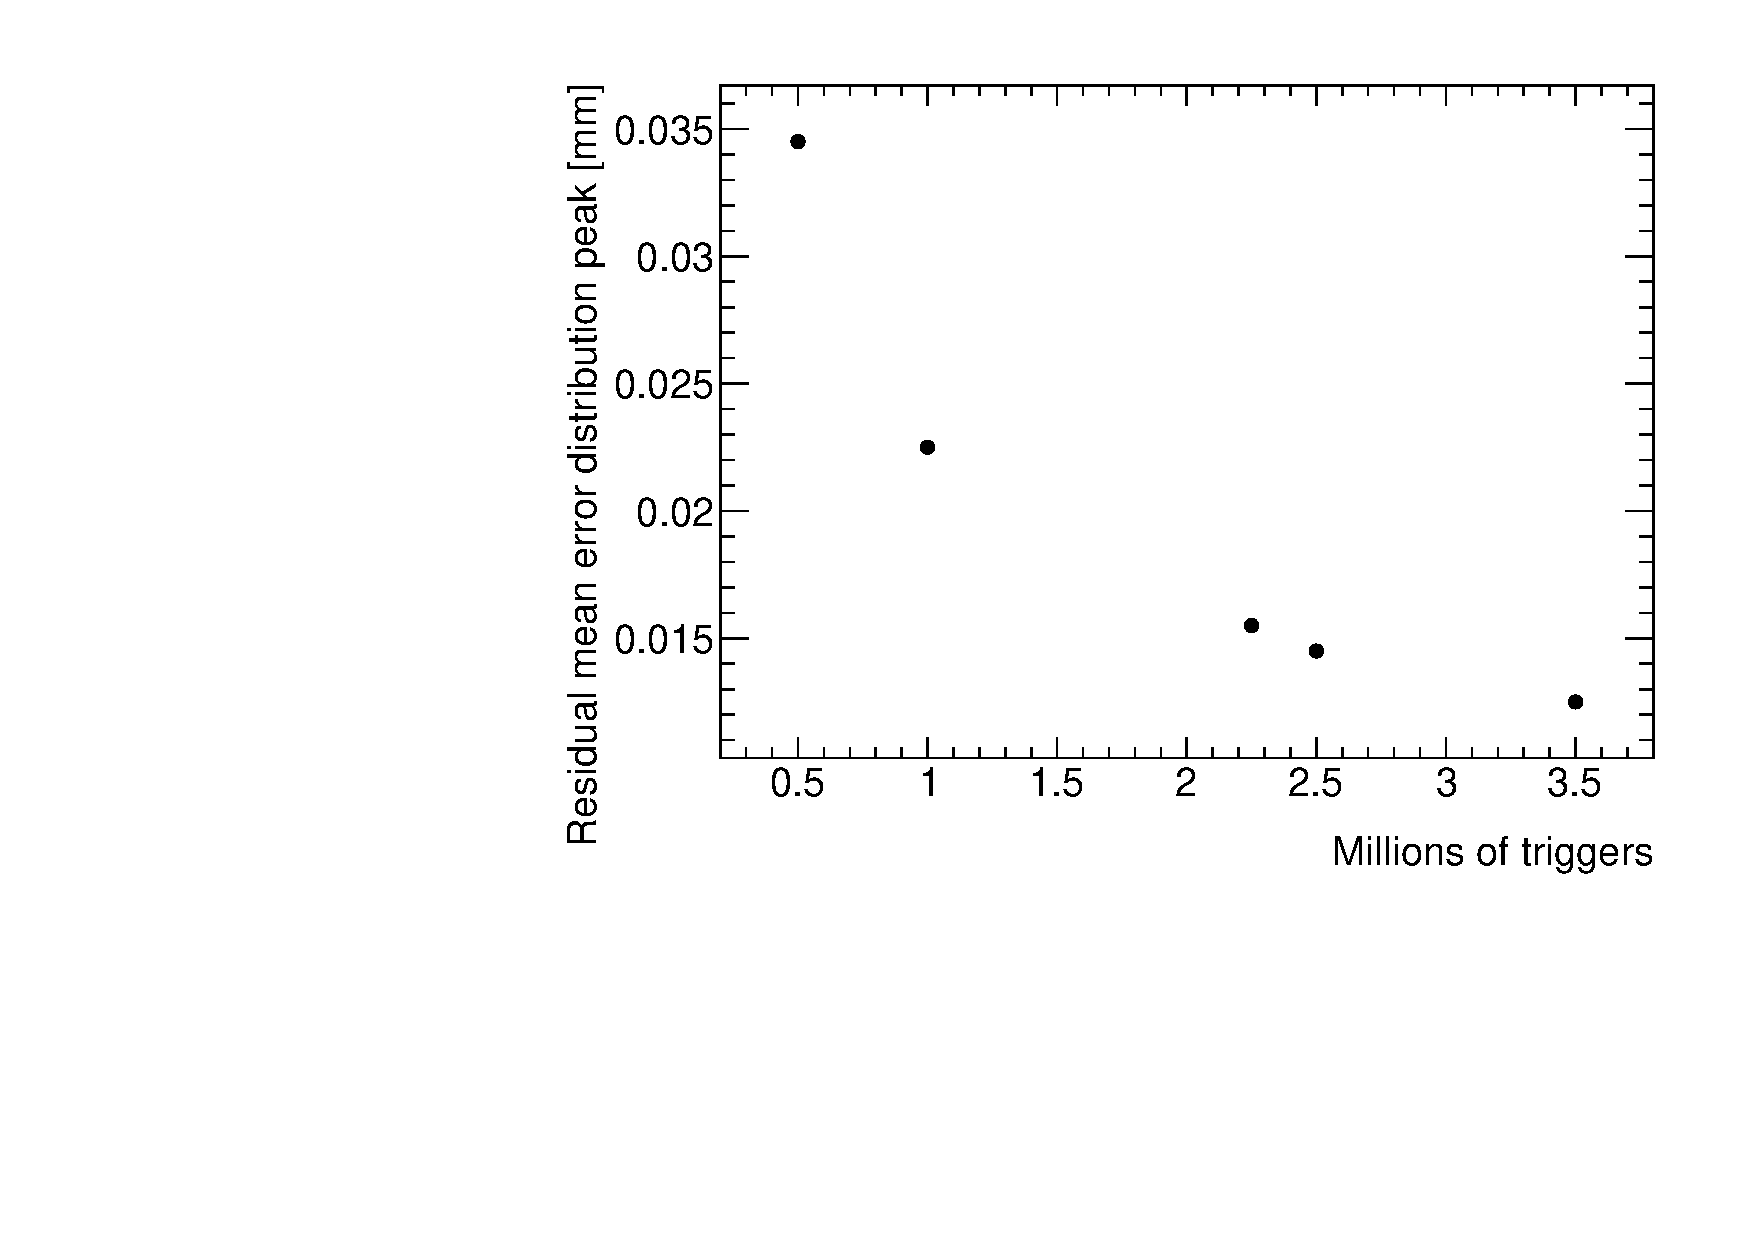
\includegraphics[width = \textwidth]{figures/figure_QS3P18_2900V_peakOfMeanErrorsDistVsTriggers_layer1_fixedlayers34.pdf}
    \caption{How the peak of the distributions of uncertainties in the residual means in regions ofinterest for tracks on layer 1 built from layers 3 and 4 changed with the number of triggers used in the analysis. The distribution falls off as $~\frac{1}{\sqrt{N}}$ as expected.}
    \label{fig:res_mean_uncert_vs_triggers}
\end{figure}

The uncertainty is already around \SI{20}{\micro\meter} at 1 million triggers, suitable for distinguishing differences in offsets of order \SI{50}{\micro\meter} as required. Although increased statistics could decrease the statistical uncertainty, it is not required for the goals of this analysis. Moreoever, the systematic uncertainty on the mean cosmics residuals is around \SI{50}{\micro\meter} so the statistical uncertainty of \SI{20}{\micro\meter} is nearly negligible.

%TODO : Include compare residual fit means for L1 F34 1 million vs 3.5 million triggers?? Do once you know how to make figures.

% ==================================================
% Appendix: Analysis Systematics %
% ==================================================

%TODO : Make mean diff plots not full page portrait. Half page would suffice. 
%TODO : Currently, section A.2 figure goes in A.3 section. Organize this once you're done writing. 
%TODO : Do I need to specify each quad? The voltage? 

\chapter[Analysis systematics]{Study of cosmics for alignment analysis systematic uncertainties}
\label{appendix:systematics}

% Sections:
% Doub gaus vs gaus -- check!
% Area bin size -- check!
% Residual distribution bin size?
%TODO 2900V vs 3100V? I think just saying strip efficiency is higher for 3100V is sufficient, although the sigmas are also smaller. But L4 F12 residual mean difference RMS is 74 um ==> Add 2900V 3100V section
% DNL
% ReClustering fit function? I think just saying I used an accepted standard is ok.

% --------------------------------------------------
\section{Residual distribution fit function}
% --------------------------------------------------
\label{appendix:systematics_res_fit_fcn}
% Edit count: 1

The distribution of residuals should be modelled by a double gaussian fit\cite{lefebvre_thesis}:

\begin{equation}
\label{eqn:doub_gaus}
G(r) = A_{s}exp\left[ \frac{-(r-\mu)^{2}}{2\sigma_s^{2}} \right] + A_{b}exp\left[ \frac{-(r-\mu)^{2}}{2\sigma_b^{2}} \right]
\end{equation}

where $r$ is the residual, $A$ is the gaussian amplitude, $\mu$ is the gaussian mean, $\sigma$ is the gaussian sigma, and the subscripts $s$ and $b$ stand for signal and background respectively. One gaussian captures the real (signal) tracks and the other captures the tracks built from noise (background). The gaussian with the smaller width is identified as the signal. 

A single gaussian fit failed less often than a double gaussian fit. The gaussian fits were performed by initially estimating the amplitude to be 100 tracks, the gaussian mean to be the histogram mean, and gaussian $\sigma$ to be the RMS. The fit range was restricted to $\pm$1 RMS from the histogram mean. The modification helped the gaussian fit capture the signal peak. An example residual distribution is shown in figure \ref{fig:double_gaussian_example_fit}. 

%TODO Why is this figure blurry?
%TODO this doesn't need to be a full page figure.

\begin{figure}
    \centering
    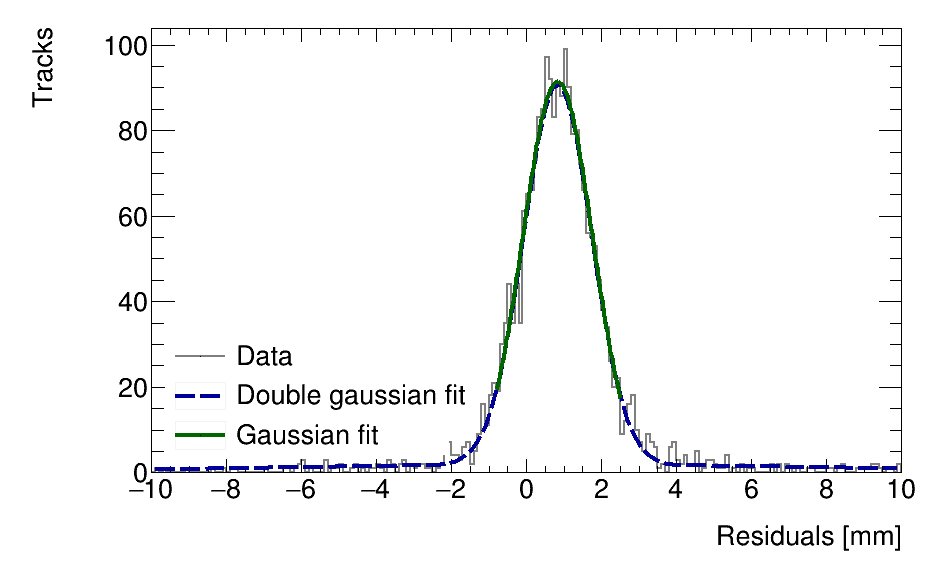
\includegraphics[width = \textwidth]{figures/figure_double_gaussian_quick_and_dirty_2900V_log_scale_gaussian_QL2C04_2900V_2021-02-08_2_xbin_10_ybin_5_100mm.png}
    \caption{Residual distribution for tracks on layer 1 built from hits on layers 3 and 4 for $x\in\left[-3.00, 97.00\right],  y\in\left[394.60, 494.60\right] mm$ for QL2.C.4 fit with a double gaussian and a single gaussian in a range of $\pm$1 RMS from the histogram mean.}
    \label{fig:double_gaussian_example_fit}
\end{figure}

For all residual distributions in \SI{100}{\milli\meter} by \SI{100}{\milli\meter} bins on layer 1 built from hits on layers 3 and 4, the difference in gaussian and double gaussian means and $\sigma$'s is shown in figure \ref{fig:double_gaussian_compare_fits}. Since the RMS of the residual mean differences distribution is less than \SI{50}{\micro\meter} the gaussian fit gave the same result within the required precision. Moreover, this is for the tracking combination with the worst extrapolation lever arm and the widest distribution of mean differences; the interpolation combinations have narrower distributions. 

The gaussian $\sigma$ should be larger than the double gaussian $\sigma$ because the gaussian distribution includes the effect of the noise tracks with large residuals, while the double gaussian models signal and background residuals separately. For this analysis, only the residual mean was important, so the systematic overestimate of the signal $\sigma$ in the gaussian fit shown on the right of figure \ref{fig:double_gaussian_compare_fits} was allowed.

\begin{figure}
    \centering
    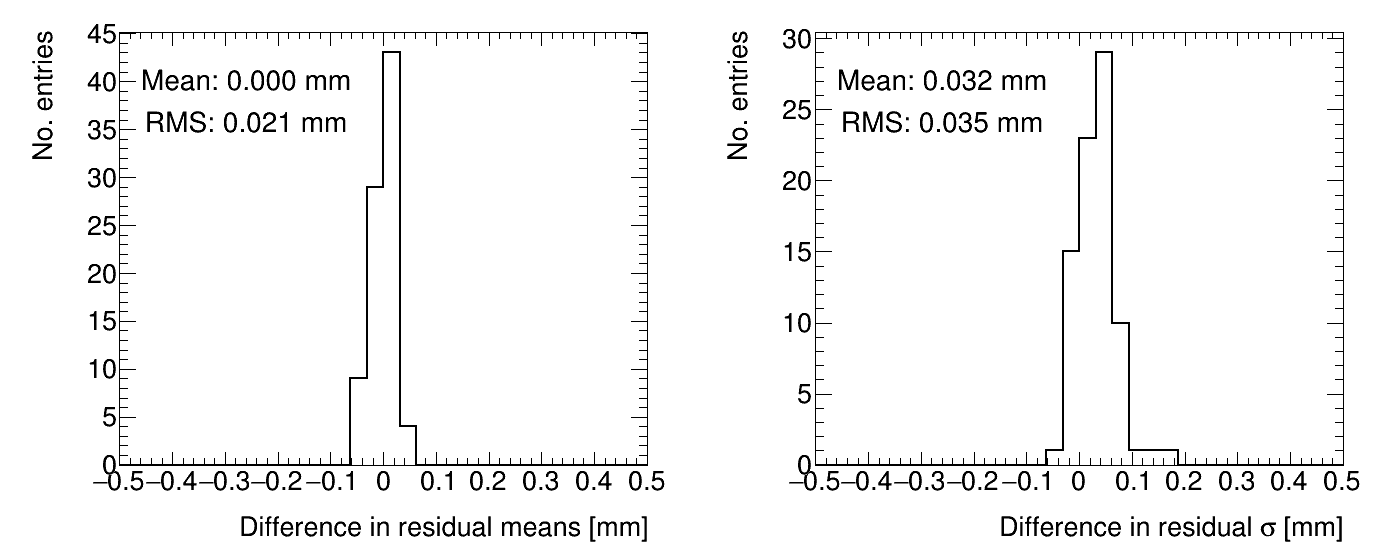
\includegraphics[width = \textwidth]{figures/figure_compare_residual_fits_QL2C04_2900V_2021-02-08_2_fit_range_mean_pm_RMS_minus_quick_and_dirty_2900V_log_scale_layer1_fixedlayers34.png}
    \caption{Difference in residual distribution means and $\sigma$'s for a gaussian and double gaussian fit, for all residual distributions in \SI{100}{\milli\meter} by \SI{100}{\milli\meter} bins on layer 1 built from hits on layers 3 and 4 for QL2.C.4, data taken at 2900 V.}
    \label{fig:double_gaussian_compare_fits}
\end{figure}

% --------------------------------------------------
\section{Area of residual distribution regions of interest}
% --------------------------------------------------
\label{appendix:systematics_bin_size}
% Edit count: 1
% DO I NEED TO EXPLAIN THIS IN MATH? I tried on June 3rd in my notes, it's complicated for such a simple thing.
% If this flies, you'll need to establish that reference frame == two fixed layers' frame as jargon in your thesis.
% Also need to establish x == perpendicular to wires; y == perpendicular to strips. ==> How do I do this consistently?
% May need to add 3100V reference if it's not already defined in your thesis.
% Define ROI as short form?

%TODO : How do I cite the distribution of rotations angles by Dylan?
The area of the region of interest in which to include tracks is primarily motivated by the misalignment model: the width of the region should be less than the scale on which the local offset is expected to change significantly. Changes in offset of order \SI{50}{\micro\meter}, the approximate position resolution of the sTGCs in the $\eta$-coordinate, are significant. In a misalignment model with an offset and rotation, only the rotation changes the local offset with respect to the x-coordinate \footnote{The effect of rotation can be modeled by assuming the recorded track position is related to the hit position by a passive rotation. The angle of rotation is the relative angle between the layer of interest and the nominal geometry. The local offset does change with respect to the track's y coordinate as well, but negligibly in the limit of small rotation angles.}.  The distribution of the as-built cathode board rotation angles shows that the RMS of the rotation angle is \SI{200}{\micro\radian} [https://indico.cern.ch/event/1035057/ PG. 18]; however, the distribution has a long tail so a typical rotation angle of \SI{1000}{\micro\radian} was used here. A rotation of \SI{1000}{\micro\radian} will cause a \SI{50}{\micro\meter} change in local offset over a change in x of \SI{50}{\centi\meter}. Therefore, the width of the region of interest should be less than \SI{500}{\milli\meter}.

Two other factors inform the width of the region. First, since the hits' x-coordinates are discrete the width in x must be larger than the pitch of the wire groups to ensure the bin will have a sufficient number of tracks fall in it. Second, more tracks will be included in a larger area so more statistics will be available for the residual distribution fit. For the bin widths wider than two wire groups, the statistics are sufficient. For each x-ray residual, the mean cosmics residual was calculated for a few different bin widths, and the difference in means plotted. Figure \ref{fig:area_bin_size_mean_diff} shows an example for QL2.C.4. The width of the distribution is on the order of \SI{50}{\micro\meter}, showing that the calculation of the residual mean is relatively robust with respect to the area of the bin. However, \SI{50}{\micro\meter} is greater than the typical statistical uncertainty on the cosmic residual of means, which ranges from \SI{10}{\micro\meter} - \SI{40}{\micro\meter} depending on the tracking combination under study. Therefore, the cosmic residual means are assigned an uncertainty of \SI{50}{\micro\meter}.
%TODO : Verity that you actually apply the 50 um uncertainty.

%TODO : This figure should have the mean and rms on it.
\begin{figure}
    \centering
    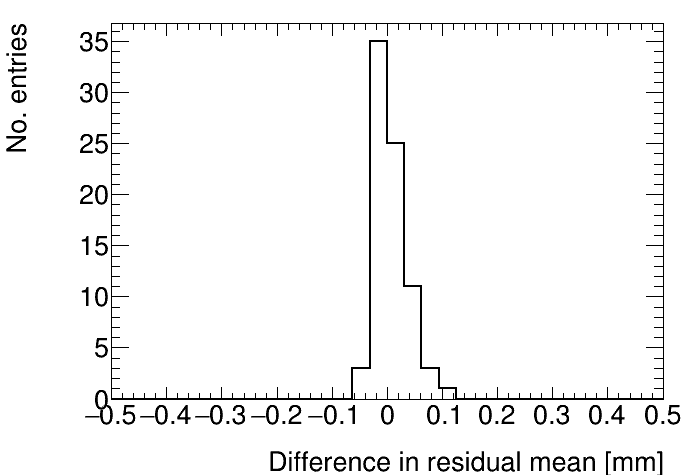
\includegraphics[width = \textwidth]{figures/compare_residual_fits_around_xrays_QL2C04_3100V_2021-05-20_100mm_width_bins_minus_QL2C04_3100V_2021-06-02_200mm_width_bins_means_difference.png}
    \caption{Difference in cosmic residual means around x-ray residuals for square bins of 100 mm width and 200 mm width for QL2.C.4.}
    \label{fig:area_bin_size_mean_diff}
\end{figure}

For this analysis, \SI{100}{\milli\meter} by \SI{100}{\milli\meter} by \SI{100}{\milli\meter} bins were used.

% --------------------------------------------------
\section{Differential non-linearity}
% --------------------------------------------------
\label{appendix:systematics_dnl}
% Edit count: 1
In this context, differential non-linearity (DNL) is when the reconstructed cluster mean is biased by the fit of the discretely sampled PDO distribution over the strips. The bias depends on the relative position of the avalanche with respect to the center of the closest strip. For a summary of DNL, refer to page 40 of Lefebvre's thesis \cite{lefebvre_thesis}. The cluster mean was corrected for DNL using the equation:
\begin{equation}
\label{eqn:dnl_corr}
y' = y + a \sin \left( 2 \pi y_{rel} \right)
\end{equation}

where $y$ is the cluster mean, $y_{rel}$ is the relative position of the cluster mean with respect to the strip's center, $a$ is the amplitude of the correction, and $y'$ is the corrected cluster mean. The amplitude can be derived by comparing the reconstructed hit position to the expected hit position, as done in Abusleme, 2016 \cite{abusleme_performance_2016}. With cosmic muons, there is no reference hit position to compare to, so track residuals were used as a proxy \cite{lefebvre_thesis}. The hallmark of the DNL effect is the periodic pattern in the residual versus $y_{rel}$ profile, and the effect of correcting the cluster means using an amplitude of \SI{50}{\micro\meter} is shown in figure \ref{fig:dnl_corr_effect}. An amplitude of \SI{50}{\micro\meter} was based on Lefebvre's estimate of the DNL amplitudes by layer, quadruplet and cluster size using exclusive cosmic muon tracks in \package{tgc\_analysis/CosmicsAnalysis}. Little variation was seen in the amplitude parameters with respect to the quadruplet tested, the layer and the cluster size so a universal correction was used.
%TODO How little is little? Check your notes.
%TODO exclusive better be defined somewhere clearly.

\begin{figure}
    \centering
    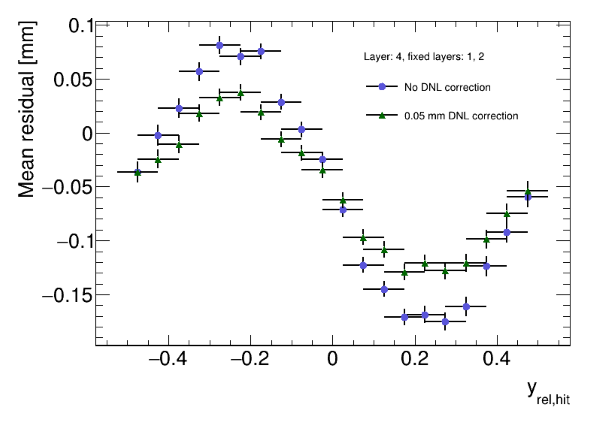
\includegraphics[width = \textwidth]{figures/figure_dnl_profiles_blue_QL2P08_3100V_2021-06-18_no_dnl_green_QL2P08_3100V_2021-06-18_2_50um_universal_DNL_layer4_fixed12.png}
    \caption{Effect applying a \SI{50}{\micro\meter} DNL correction to the cluster means on the residual vs $y_{rel}$ distribution for tracks built from layers 1 and 2 and extrapolated to layer 4 for QL2.P.8.}
    \label{fig:dnl_corr_effect}
\end{figure} 

Although the correction is not large enough in this case, the figure shows that the correction does reduce the DNL effect. Slightly better performance is seen in the interpolation tracking combinations where the quality of the residuals is better. DNL corrections for cosmic muon data are difficult because the DNL effect is obscured by the effect of misalignments and noise. Misalignments cause the center of the sine pattern in figure \ref{fig:dnl_corr_effect} to be shifted off of zero, since the mean of residuals is shifted.

In figure \ref{fig:dnl_compare_fits}, it is apparent that the effect of the DNL correction on the mean of the residual distribution in \SI{100}{\milli\meter} by \SI{100}{\milli\meter} areas is on the order of micrometers in the worst extrapolation case. Although the $\sigma$'s of the residual distributions shrink with the DNL correction, the mean is the parameter of interest. Therefore, for this analysis DNL was not corrected for.

\begin{figure}
    \centering
    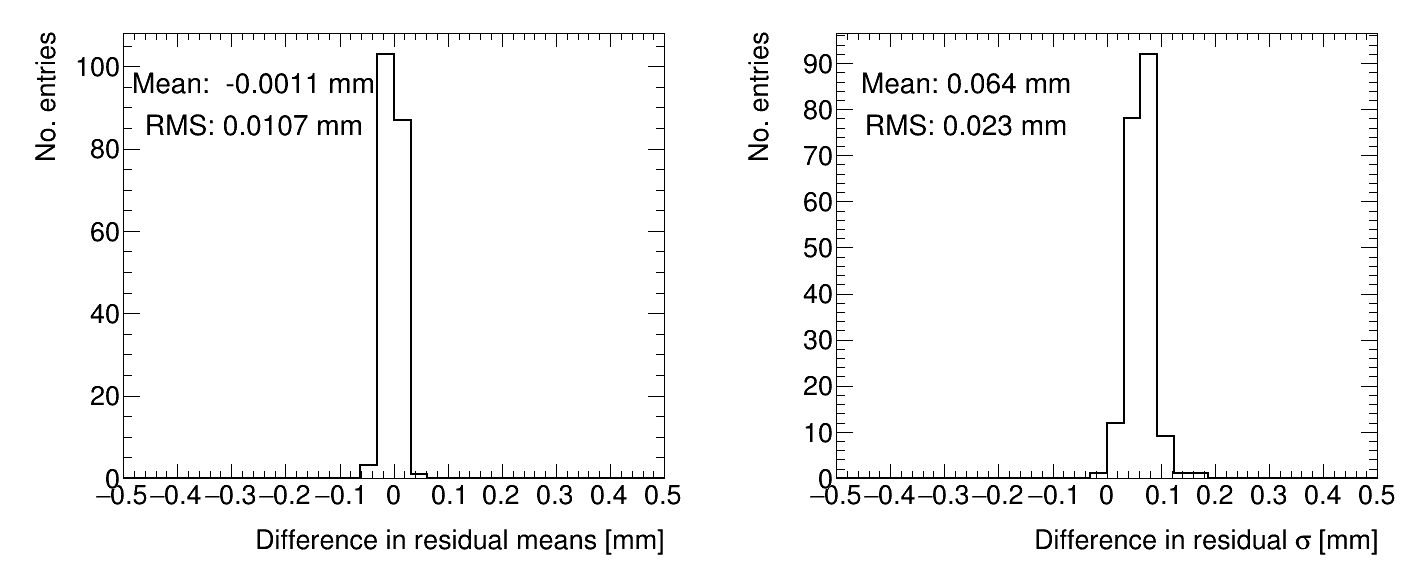
\includegraphics[width = \textwidth]{figures/figure_compare_residual_fits_QL2P08_3100V_2021-06-18_no_dnl_minus_QL2P08_3100V_2021-06-18_2_50um_universal_DNL_layer4_fixedlayers12.png}
    \caption{Difference in residual distribution means and $\sigma$'s with and without DNL correction for residuals on layer 4 from reference layers 1 and 2 for QL2.P.8.}
    \label{fig:dnl_compare_fits}
\end{figure}

































% GLOSSARIES (Lists of definitions, abbreviations, symbols, etc. provided by the glossaries-extra package)
% -----------------------------
% \printglossaries
% \cleardoublepage
% \phantomsection		% allows hyperref to link to the correct page

%----------------------------------------------------------------------
\end{document} % end of logical document
